\PassOptionsToPackage{unicode=true}{hyperref} % options for packages loaded elsewhere
\PassOptionsToPackage{hyphens}{url}
%
\documentclass[11pt,ignorenonframetext,]{beamer}
\setbeamertemplate{caption}[numbered]
\setbeamertemplate{caption label separator}{: }
\setbeamercolor{caption name}{fg=normal text.fg}
\beamertemplatenavigationsymbolsempty
\usepackage{lmodern}
\usepackage{amssymb,amsmath}
\usepackage{ifxetex,ifluatex}
\usepackage{fixltx2e} % provides \textsubscript
\ifnum 0\ifxetex 1\fi\ifluatex 1\fi=0 % if pdftex
  \usepackage[T1]{fontenc}
  \usepackage[utf8]{inputenc}
  \usepackage{textcomp} % provides euro and other symbols
\else % if luatex or xelatex
  \usepackage{unicode-math}
  \defaultfontfeatures{Ligatures=TeX,Scale=MatchLowercase}
\fi
\usetheme[]{metropolis}
% use upquote if available, for straight quotes in verbatim environments
\IfFileExists{upquote.sty}{\usepackage{upquote}}{}
% use microtype if available
\IfFileExists{microtype.sty}{%
\usepackage[]{microtype}
\UseMicrotypeSet[protrusion]{basicmath} % disable protrusion for tt fonts
}{}
\IfFileExists{parskip.sty}{%
\usepackage{parskip}
}{% else
\setlength{\parindent}{0pt}
\setlength{\parskip}{6pt plus 2pt minus 1pt}
}
\usepackage{hyperref}
\hypersetup{
            pdftitle={Lecture 16},
            pdfborder={0 0 0},
            breaklinks=true}
\urlstyle{same}  % don't use monospace font for urls
\newif\ifbibliography
\usepackage{color}
\usepackage{fancyvrb}
\newcommand{\VerbBar}{|}
\newcommand{\VERB}{\Verb[commandchars=\\\{\}]}
\DefineVerbatimEnvironment{Highlighting}{Verbatim}{commandchars=\\\{\}}
% Add ',fontsize=\small' for more characters per line
\newenvironment{Shaded}{}{}
\newcommand{\AlertTok}[1]{\textcolor[rgb]{1.00,0.00,0.00}{\textbf{#1}}}
\newcommand{\AnnotationTok}[1]{\textcolor[rgb]{0.38,0.63,0.69}{\textbf{\textit{#1}}}}
\newcommand{\AttributeTok}[1]{\textcolor[rgb]{0.49,0.56,0.16}{#1}}
\newcommand{\BaseNTok}[1]{\textcolor[rgb]{0.25,0.63,0.44}{#1}}
\newcommand{\BuiltInTok}[1]{#1}
\newcommand{\CharTok}[1]{\textcolor[rgb]{0.25,0.44,0.63}{#1}}
\newcommand{\CommentTok}[1]{\textcolor[rgb]{0.38,0.63,0.69}{\textit{#1}}}
\newcommand{\CommentVarTok}[1]{\textcolor[rgb]{0.38,0.63,0.69}{\textbf{\textit{#1}}}}
\newcommand{\ConstantTok}[1]{\textcolor[rgb]{0.53,0.00,0.00}{#1}}
\newcommand{\ControlFlowTok}[1]{\textcolor[rgb]{0.00,0.44,0.13}{\textbf{#1}}}
\newcommand{\DataTypeTok}[1]{\textcolor[rgb]{0.56,0.13,0.00}{#1}}
\newcommand{\DecValTok}[1]{\textcolor[rgb]{0.25,0.63,0.44}{#1}}
\newcommand{\DocumentationTok}[1]{\textcolor[rgb]{0.73,0.13,0.13}{\textit{#1}}}
\newcommand{\ErrorTok}[1]{\textcolor[rgb]{1.00,0.00,0.00}{\textbf{#1}}}
\newcommand{\ExtensionTok}[1]{#1}
\newcommand{\FloatTok}[1]{\textcolor[rgb]{0.25,0.63,0.44}{#1}}
\newcommand{\FunctionTok}[1]{\textcolor[rgb]{0.02,0.16,0.49}{#1}}
\newcommand{\ImportTok}[1]{#1}
\newcommand{\InformationTok}[1]{\textcolor[rgb]{0.38,0.63,0.69}{\textbf{\textit{#1}}}}
\newcommand{\KeywordTok}[1]{\textcolor[rgb]{0.00,0.44,0.13}{\textbf{#1}}}
\newcommand{\NormalTok}[1]{#1}
\newcommand{\OperatorTok}[1]{\textcolor[rgb]{0.40,0.40,0.40}{#1}}
\newcommand{\OtherTok}[1]{\textcolor[rgb]{0.00,0.44,0.13}{#1}}
\newcommand{\PreprocessorTok}[1]{\textcolor[rgb]{0.74,0.48,0.00}{#1}}
\newcommand{\RegionMarkerTok}[1]{#1}
\newcommand{\SpecialCharTok}[1]{\textcolor[rgb]{0.25,0.44,0.63}{#1}}
\newcommand{\SpecialStringTok}[1]{\textcolor[rgb]{0.73,0.40,0.53}{#1}}
\newcommand{\StringTok}[1]{\textcolor[rgb]{0.25,0.44,0.63}{#1}}
\newcommand{\VariableTok}[1]{\textcolor[rgb]{0.10,0.09,0.49}{#1}}
\newcommand{\VerbatimStringTok}[1]{\textcolor[rgb]{0.25,0.44,0.63}{#1}}
\newcommand{\WarningTok}[1]{\textcolor[rgb]{0.38,0.63,0.69}{\textbf{\textit{#1}}}}
% Prevent slide breaks in the middle of a paragraph:
\widowpenalties 1 10000
\raggedbottom
\setbeamertemplate{part page}{
\centering
\begin{beamercolorbox}[sep=16pt,center]{part title}
  \usebeamerfont{part title}\insertpart\par
\end{beamercolorbox}
}
\setbeamertemplate{section page}{
\centering
\begin{beamercolorbox}[sep=12pt,center]{part title}
  \usebeamerfont{section title}\insertsection\par
\end{beamercolorbox}
}
\setbeamertemplate{subsection page}{
\centering
\begin{beamercolorbox}[sep=8pt,center]{part title}
  \usebeamerfont{subsection title}\insertsubsection\par
\end{beamercolorbox}
}
\AtBeginPart{
  \frame{\partpage}
}
\AtBeginSection{
  \ifbibliography
  \else
    \frame{\sectionpage}
  \fi
}
\AtBeginSubsection{
  \frame{\subsectionpage}
}
\setlength{\emergencystretch}{3em}  % prevent overfull lines
\providecommand{\tightlist}{%
  \setlength{\itemsep}{0pt}\setlength{\parskip}{0pt}}
\setcounter{secnumdepth}{0}

% set default figure placement to htbp
\makeatletter
\def\fps@figure{htbp}
\makeatother

\usepackage{geometry}
\usepackage{graphicx}

\usepackage{bbold}
\usepackage{lmodern}


\usepackage{url}		% produces hyperlinks

\usepackage{colortbl}	% allows for color usage in tables
\usepackage{multirow}	% allows for rows that span multiple rows in tables

\usepackage{color}          	% gives color options
\usepackage{xcolor}		% this package has a variety of color options

\usepackage{multicol}
\usepackage{textcomp}

\usepackage{setspace}
\usepackage{changepage}
\usepackage{isotope}

\singlespacing

%%%%%%%%%%%%%%%%
% Small code output
%%%%%%%%%%%%%%%%

%% change fontsize of R code

\makeatletter
\@ifundefined{Shaded}{\newenvironment{Shaded}{}{}}{}
\makeatother


\let\oldShaded\Shaded
\let\endoldShaded\endShaded
\renewenvironment{Shaded}{\footnotesize\begin{spacing}{0.9}\oldShaded}{\endoldShaded\end{spacing}}

%% change fontsize of output
\let\oldverbatim\verbatim
\let\endoldverbatim\endverbatim
\renewenvironment{verbatim}{\footnotesize\begin{spacing}{0.9}\oldverbatim}{\endoldverbatim\end{spacing}}


\newcommand{\tinyoutput}{
  \renewenvironment{Shaded}{\tiny\begin{spacing}{0.9}\oldShaded}{\endoldShaded\end{spacing}}
  \renewenvironment{verbatim}{\tiny\begin{spacing}{0.9}\oldverbatim}{\endoldverbatim\end{spacing}}
}

\newcommand{\scriptoutput}{
  \renewenvironment{Shaded}{\scriptsize\begin{spacing}{0.9}\oldShaded}{\endoldShaded\end{spacing}}
  \renewenvironment{verbatim}{\scriptsize\begin{spacing}{0.9}\oldverbatim}{\endoldverbatim\end{spacing}}
}

\newcommand{\footnoteoutput}{
  \renewenvironment{Shaded}{\footnotesize\begin{spacing}{0.9}\oldShaded}{\endoldShaded\end{spacing}}
  \renewenvironment{verbatim}{\footnotesize\begin{spacing}{0.9}\oldverbatim}{\endoldverbatim\end{spacing}}
}

%\newcommand{\verbatimfont}[1]{\renewcommand{\verbatim@font}{\ttfamily#1}}


%%%%%%%%%%%%%%%%
% Custom Colors
%%%%%%%%%%%%%%%%

\definecolor{redhl}{rgb}{0.98,0.29,0.28}
\definecolor{yellowhl}{rgb}{0.98,0.87,0.28}


\xdefinecolor{oiBlue}{rgb}{0.15, 0.35, 0.55}
\xdefinecolor{gray}{rgb}{0.5, 0.5, 0.5}
\xdefinecolor{darkGray}{rgb}{0.3, 0.3, 0.3}
\xdefinecolor{darkerGray}{rgb}{0.2, 0.2, 0.2}
\xdefinecolor{rubineRed}{rgb}{0.89,0,0.30}
\xdefinecolor{linkCol}{rgb}{0.11,0.49,0.95}	
\xdefinecolor{irishGreen}{rgb}{0,0.60,0}	
\xdefinecolor{darkturquoise}{rgb}{0.44, 0.58, 0.86}
\definecolor{lightGreen}{rgb}{0.533,0.765,0.42}
%\xdefinecolor{hlblue}{rgb}{0.051,0.65,1}
\xdefinecolor{hlblue}{rgb}{ 0.055, 0.639, 0.831}
\definecolor{light}{rgb}{.337,.608,.741}
\definecolor{dark}{rgb}{.337,.608,.741}

\definecolor{cpink}{rgb}{0.93, 0.23, 0.51}

%%%%%%%%%%%%%%%%
% Custom Commands
%%%%%%%%%%%%%%%%

% text colors
\newcommand{\red}[1]{\textit{\textcolor{rubineRed}{#1}}}
\newcommand{\orange}[1]{\textit{\textcolor{orange}{#1}}}
\newcommand{\pink}[1]{\textit{\textcolor{rubineRed!90!white!50}{#1}}}
\newcommand{\green}[1]{\textit{\textcolor{irishGreen}{#1}}}
\newcommand{\blue}[1]{\textit{\textcolor{darkturquoise}{#1}}}
\newcommand{\light}[1]{\textcolor{light}{\textbf{#1}}}
\newcommand{\dark}[1]{\textcolor{dark}{#1}}
\newcommand{\gray}[1]{\textcolor{gray}{#1}}


% mail
\newcommand{\mail}[1]{\href{mailto:#1}{\textit{\textcolor{linkCol}{#1}}}}

% highlighting: hl, hlGr, mathhl
\newcommand{\hl}[1]{\textit{\textcolor{hlblue}{#1}}}
\newcommand{\hlGr}[1]{\textit{\textcolor{lightGreen}{#1}}}
\newcommand{\hlRd}[1]{\textit{\textcolor{rubineRed}{#1}}}
\newcommand{\mathhl}[1]{\textcolor{hlblue}{\ensuremath{#1}}}
\newcommand{\hlr}[1]{\fcolorbox{redhl}{white}{$\displaystyle #1$}}
\newcommand{\hly}[1]{\fcolorbox{yellowhl}{white}{$\displaystyle #1$}}


\newcommand{\vvfill}{\vskip0pt plus 1filll}

\DeclareMathOperator*{\argmin}{arg\,min}
\DeclareMathOperator*{\argmax}{arg\,max}

\title{Lecture 16}
\providecommand{\subtitle}[1]{}
\subtitle{Spatial Data and Cartography (Part 2)}
\date{3/22/2018}

\begin{document}
\frame{\titlepage}

\hypertarget{plotting}{%
\section{Plotting}\label{plotting}}

\begin{frame}[fragile,t]{Example Data - NC SIDS}
\protect\hypertarget{example-data---nc-sids}{}

\scriptoutput

\begin{Shaded}
\begin{Highlighting}[]
\NormalTok{nc =}\StringTok{ }\KeywordTok{st_read}\NormalTok{(}\KeywordTok{system.file}\NormalTok{(}\StringTok{"shape/nc.shp"}\NormalTok{, }\DataTypeTok{package=}\StringTok{"sf"}\NormalTok{), }\DataTypeTok{quiet =} \OtherTok{TRUE}\NormalTok{) }\OperatorTok\StringTok{ }
\StringTok{  }\KeywordTok{select}\NormalTok{(}\OperatorTok{-}\NormalTok{(AREA}\OperatorTok{:}\NormalTok{CNTY_ID), }\OperatorTok{-}\NormalTok{(FIPS}\OperatorTok{:}\NormalTok{CRESS_ID))}

\KeywordTok{tbl_df}\NormalTok{(nc)}
\NormalTok{## # A tibble: 100 x 8}
\NormalTok{##    NAME  BIR74 SID74 NWBIR74 BIR79 SID79 NWBIR79                  geometry}
\NormalTok{##    <fct> <dbl> <dbl>   <dbl> <dbl> <dbl>   <dbl>        <MULTIPOLYGON [°]>}
\NormalTok{##  1 Ashe  1091.    1.     10. 1364.    0.     19. (((-81.47276 36.23436, -~}
\NormalTok{##  2 Alle~  487.    0.     10.  542.    3.     12. (((-81.23989 36.36536, -~}
\NormalTok{##  3 Surry 3188.    5.    208. 3616.    6.    260. (((-80.45634 36.24256, -~}
\NormalTok{##  4 Curr~  508.    1.    123.  830.    2.    145. (((-76.00897 36.3196, -7~}
\NormalTok{##  5 Nort~ 1421.    9.   1066. 1606.    3.   1197. (((-77.21767 36.24098, -~}
\NormalTok{##  6 Hert~ 1452.    7.    954. 1838.    5.   1237. (((-76.74506 36.23392, -~}
\NormalTok{##  7 Camd~  286.    0.    115.  350.    2.    139. (((-76.00897 36.3196, -7~}
\NormalTok{##  8 Gates  420.    0.    254.  594.    2.    371. (((-76.56251 36.34057, -~}
\NormalTok{##  9 Warr~  968.    4.    748. 1190.    2.    844. (((-78.30876 36.26004, -~}
\NormalTok{## 10 Stok~ 1612.    1.    160. 2038.    5.    176. (((-80.02567 36.25023, -~}
\NormalTok{## # ... with 90 more rows}
\end{Highlighting}
\end{Shaded}

\end{frame}

\begin{frame}[fragile,t]{Base Plots}
\protect\hypertarget{base-plots}{}

\scriptoutput

\begin{Shaded}
\begin{Highlighting}[]
\KeywordTok{plot}\NormalTok{(nc)}
\end{Highlighting}
\end{Shaded}

\begin{center}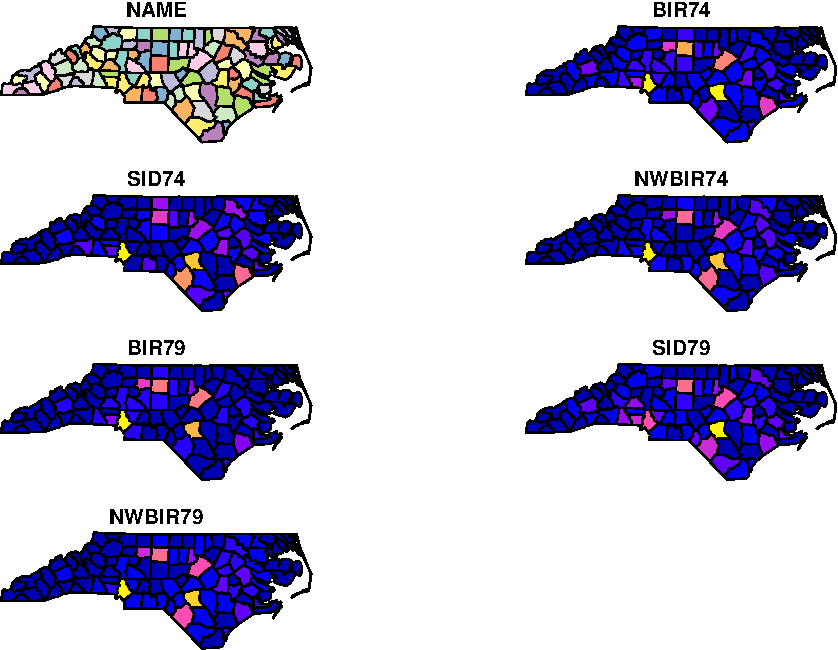
\includegraphics[width=0.8\textwidth]{Lec16_files/figure-beamer/unnamed-chunk-2-1} \end{center}

\end{frame}

\begin{frame}[fragile,t]{Geometry Plot}
\protect\hypertarget{geometry-plot}{}

\scriptoutput

\begin{Shaded}
\begin{Highlighting}[]
\KeywordTok{plot}\NormalTok{(}\KeywordTok{st_geometry}\NormalTok{(nc), }\DataTypeTok{axes=}\OtherTok{TRUE}\NormalTok{)}
\end{Highlighting}
\end{Shaded}

\begin{center}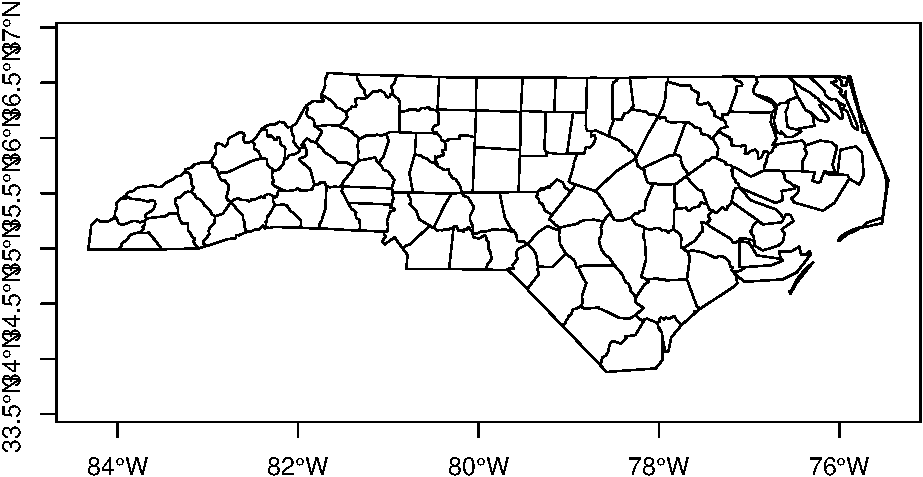
\includegraphics[width=\textwidth]{Lec16_files/figure-beamer/unnamed-chunk-3-1} \end{center}

\end{frame}

\begin{frame}[fragile,t]{Graticules}
\protect\hypertarget{graticules}{}

\scriptoutput

\begin{Shaded}
\begin{Highlighting}[]
\KeywordTok{plot}\NormalTok{(nc[,}\StringTok{"SID79"}\NormalTok{], }\DataTypeTok{graticule=}\KeywordTok{st_crs}\NormalTok{(nc), }\DataTypeTok{axes=}\OtherTok{TRUE}\NormalTok{)}
\end{Highlighting}
\end{Shaded}

\begin{center}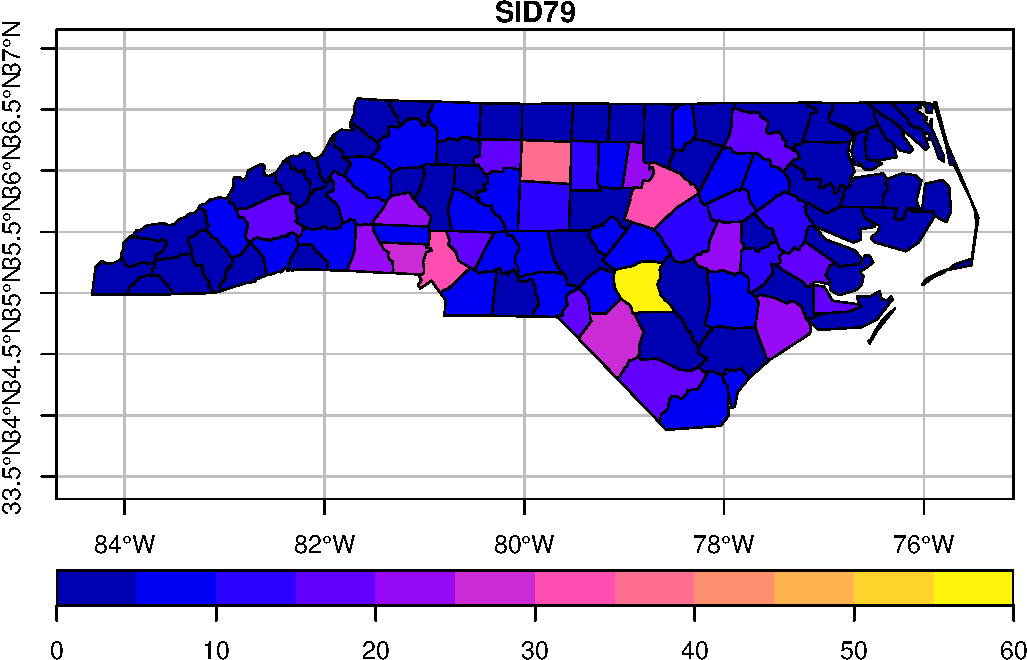
\includegraphics[width=\textwidth]{Lec16_files/figure-beamer/unnamed-chunk-4-1} \end{center}

\end{frame}

\begin{frame}[fragile,t]{Graticules (EPSG:3631)}
\protect\hypertarget{graticules-epsg3631}{}

\scriptoutput

\begin{Shaded}
\begin{Highlighting}[]
\KeywordTok{plot}\NormalTok{(}\KeywordTok{st_transform}\NormalTok{(nc[,}\StringTok{"SID79"}\NormalTok{], }\DecValTok{3631}\NormalTok{), }\DataTypeTok{graticule=}\KeywordTok{st_crs}\NormalTok{(nc), }\DataTypeTok{axes=}\OtherTok{TRUE}\NormalTok{)}
\end{Highlighting}
\end{Shaded}

\begin{center}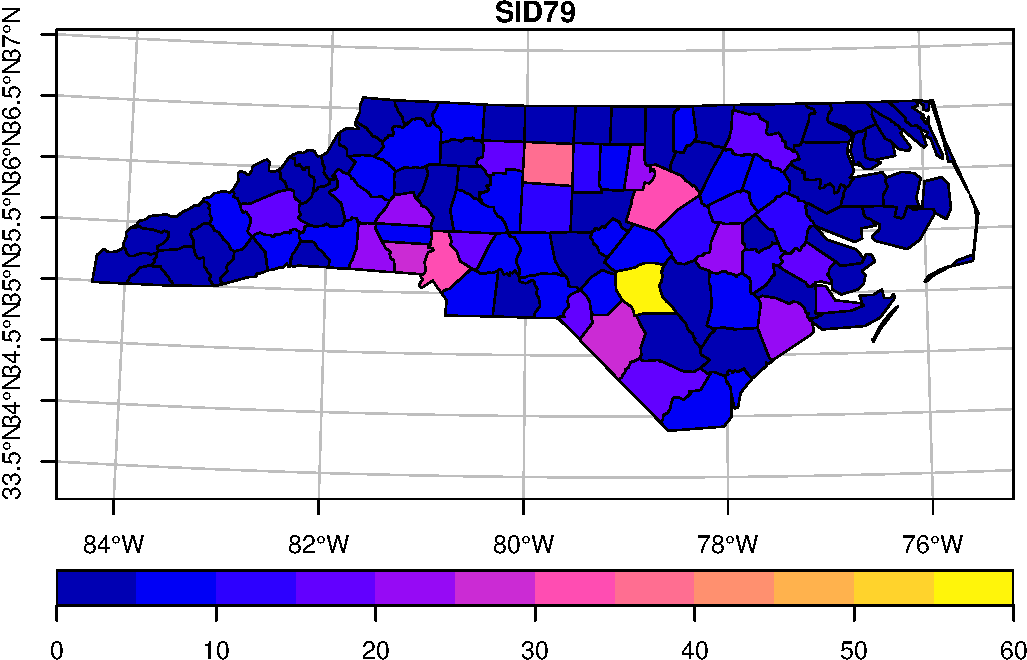
\includegraphics[width=\textwidth]{Lec16_files/figure-beamer/unnamed-chunk-5-1} \end{center}

\end{frame}

\begin{frame}[fragile,t]{ggplot2 (dev)}
\protect\hypertarget{ggplot2-dev}{}

\scriptoutput

\begin{Shaded}
\begin{Highlighting}[]
\NormalTok{devtools}\OperatorTok{::}\KeywordTok{install_github}\NormalTok{(}\StringTok{"tidyverse/ggplot2"}\NormalTok{)}
\end{Highlighting}
\end{Shaded}

\begin{Shaded}
\begin{Highlighting}[]
\KeywordTok{ggplot}\NormalTok{(nc) }\OperatorTok{+}\StringTok{ }
\StringTok{  }\KeywordTok{geom_sf}\NormalTok{(}\KeywordTok{aes}\NormalTok{(}\DataTypeTok{fill=}\NormalTok{SID79))}
\end{Highlighting}
\end{Shaded}

\begin{center}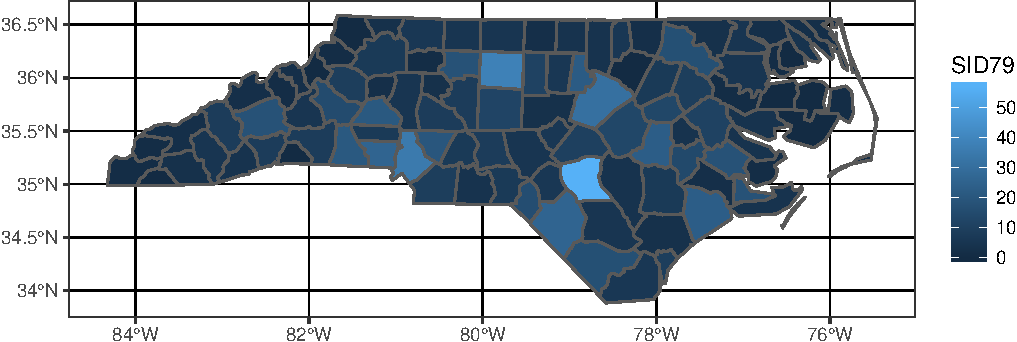
\includegraphics[width=\textwidth]{Lec16_files/figure-beamer/unnamed-chunk-7-1} \end{center}

\end{frame}

\begin{frame}[fragile,t]{ggplot2 + projections}
\protect\hypertarget{ggplot2-projections}{}

\scriptoutput

\begin{Shaded}
\begin{Highlighting}[]
\KeywordTok{ggplot}\NormalTok{(}\KeywordTok{st_transform}\NormalTok{(nc, }\DecValTok{3631}\NormalTok{)) }\OperatorTok{+}\StringTok{ }
\StringTok{  }\KeywordTok{geom_sf}\NormalTok{(}\KeywordTok{aes}\NormalTok{(}\DataTypeTok{fill=}\NormalTok{SID79 }\OperatorTok{/}\StringTok{ }\NormalTok{BIR79))}
\end{Highlighting}
\end{Shaded}

\begin{center}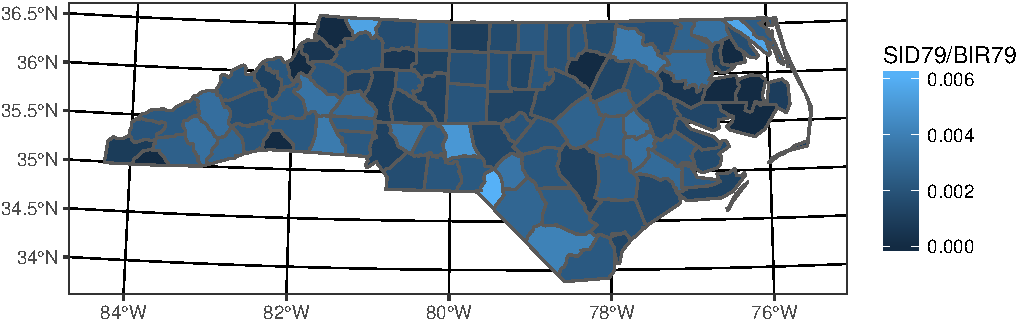
\includegraphics[width=\textwidth]{Lec16_files/figure-beamer/unnamed-chunk-8-1} \end{center}

\end{frame}

\begin{frame}[fragile]{Example Data - Meuse}
\protect\hypertarget{example-data---meuse}{}

\scriptoutput

\begin{Shaded}
\begin{Highlighting}[]
\KeywordTok{data}\NormalTok{(meuse, meuse.riv, }\DataTypeTok{package=}\StringTok{"sp"}\NormalTok{)}

\NormalTok{meuse =}\StringTok{ }\KeywordTok{st_as_sf}\NormalTok{(meuse, }\DataTypeTok{coords=}\KeywordTok{c}\NormalTok{(}\StringTok{"x"}\NormalTok{, }\StringTok{"y"}\NormalTok{), }\DataTypeTok{crs=}\DecValTok{28992}\NormalTok{)}
\NormalTok{meuse_riv =}\StringTok{ }\KeywordTok{st_polygon}\NormalTok{(}\KeywordTok{list}\NormalTok{(meuse.riv)) }\OperatorTok\StringTok{ }\KeywordTok{st_sfc}\NormalTok{() }\OperatorTok\StringTok{ }\KeywordTok{st_set_crs}\NormalTok{(}\DecValTok{28992}\NormalTok{)}

\KeywordTok{tbl_df}\NormalTok{(meuse)}
\NormalTok{## # A tibble: 155 x 13}
\NormalTok{##    cadmium copper  lead  zinc  elev    dist    om ffreq soil  lime }
\NormalTok{##  *   <dbl>  <dbl> <dbl> <dbl> <dbl>   <dbl> <dbl> <fct> <fct> <fct>}
\NormalTok{##  1   11.7     85.  299. 1022.  7.91 0.00136 13.6  1     1     1    }
\NormalTok{##  2    8.60    81.  277. 1141.  6.98 0.0122  14.0  1     1     1    }
\NormalTok{##  3    6.50    68.  199.  640.  7.80 0.103   13.0  1     1     1    }
\NormalTok{##  4    2.60    81.  116.  257.  7.66 0.190    8.00 1     2     0    }
\NormalTok{##  5    2.80    48.  117.  269.  7.48 0.277    8.70 1     2     0    }
\NormalTok{##  6    3.00    61.  137.  281.  7.79 0.364    7.80 1     2     0    }
\NormalTok{##  7    3.20    31.  132.  346.  8.22 0.190    9.20 1     2     0    }
\NormalTok{##  8    2.80    29.  150.  406.  8.49 0.0922   9.50 1     1     0    }
\NormalTok{##  9    2.40    37.  133.  347.  8.67 0.185   10.6  1     1     0    }
\NormalTok{## 10    1.60    24.   80.  183.  9.05 0.310    6.30 1     2     0    }
\NormalTok{## # ... with 145 more rows, and 3 more variables: landuse <fct>,}
\NormalTok{## #   dist.m <dbl>, geometry <POINT [m]>}
\end{Highlighting}
\end{Shaded}

\end{frame}

\begin{frame}[fragile,t]{Meuse}
\protect\hypertarget{meuse}{}

\scriptoutput

\begin{Shaded}
\begin{Highlighting}[]
\KeywordTok{plot}\NormalTok{(meuse, }\DataTypeTok{pch=}\DecValTok{16}\NormalTok{)}
\end{Highlighting}
\end{Shaded}

\begin{center}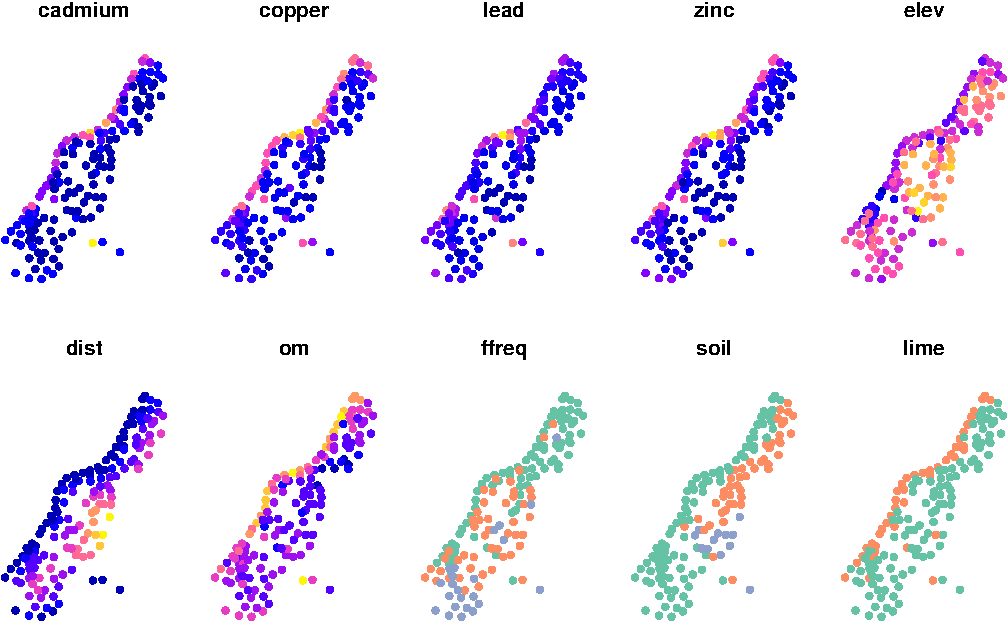
\includegraphics[width=\textwidth]{Lec16_files/figure-beamer/unnamed-chunk-10-1} \end{center}

\end{frame}

\begin{frame}[fragile,t]{Layering plots}
\protect\hypertarget{layering-plots}{}

\scriptoutput

\begin{Shaded}
\begin{Highlighting}[]
\KeywordTok{plot}\NormalTok{(meuse[,}\StringTok{"lead"}\NormalTok{], }\DataTypeTok{pch=}\DecValTok{16}\NormalTok{, }\DataTypeTok{axes=}\OtherTok{TRUE}\NormalTok{)}
\KeywordTok{plot}\NormalTok{(meuse_riv, }\DataTypeTok{col=}\KeywordTok{adjustcolor}\NormalTok{(}\StringTok{"lightblue"}\NormalTok{, }\DataTypeTok{alpha.f=}\FloatTok{0.5}\NormalTok{), }\DataTypeTok{add=}\OtherTok{TRUE}\NormalTok{, }\DataTypeTok{border =} \OtherTok{NA}\NormalTok{)}
\end{Highlighting}
\end{Shaded}

\begin{center}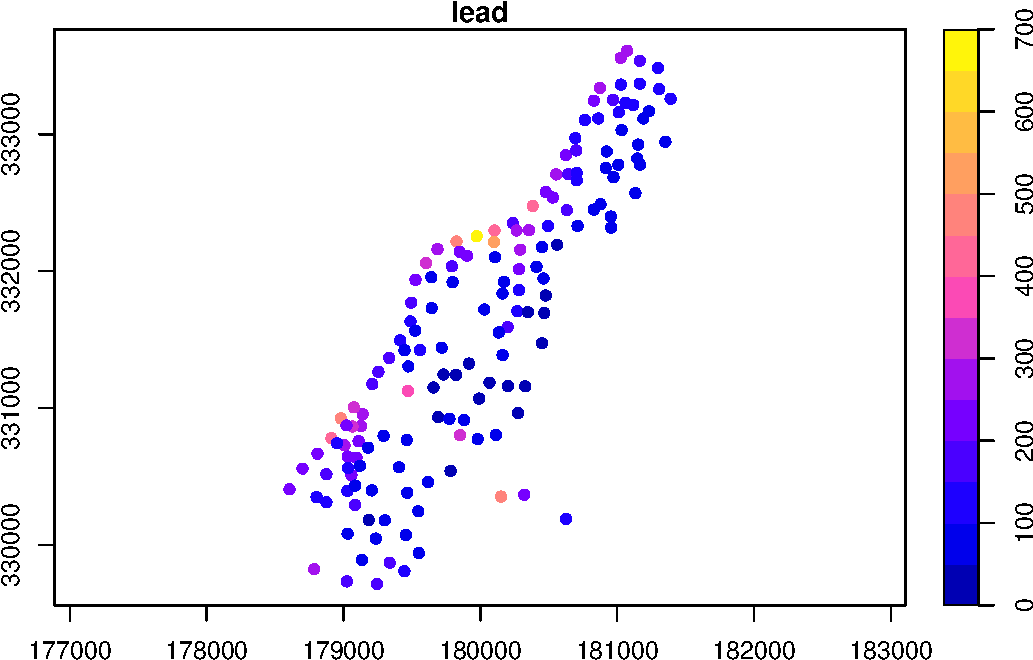
\includegraphics[width=\textwidth]{Lec16_files/figure-beamer/unnamed-chunk-11-1} \end{center}

\end{frame}

\begin{frame}[fragile,t]{Layering plots (oops)}
\protect\hypertarget{layering-plots-oops}{}

\scriptoutput

\begin{Shaded}
\begin{Highlighting}[]
\KeywordTok{plot}\NormalTok{(meuse, }\DataTypeTok{pch=}\DecValTok{16}\NormalTok{)}
\KeywordTok{plot}\NormalTok{(meuse_riv, }\DataTypeTok{col=}\KeywordTok{adjustcolor}\NormalTok{(}\StringTok{"lightblue"}\NormalTok{, }\DataTypeTok{alpha.f=}\FloatTok{0.5}\NormalTok{), }\DataTypeTok{add=}\OtherTok{TRUE}\NormalTok{, }\DataTypeTok{border =} \OtherTok{NA}\NormalTok{)}
\end{Highlighting}
\end{Shaded}

\begin{center}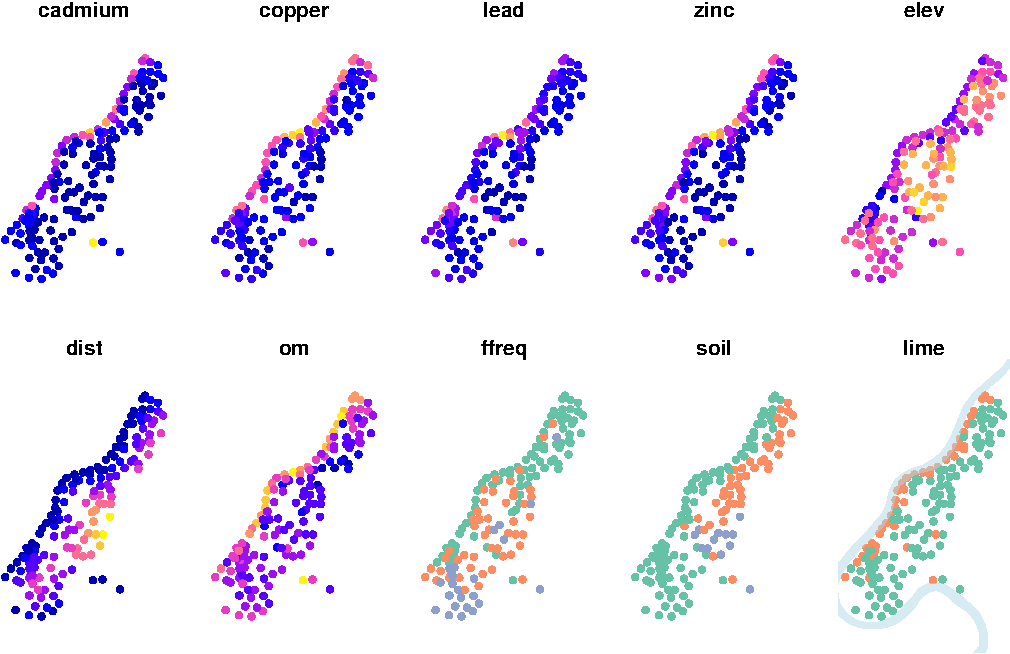
\includegraphics[width=\textwidth]{Lec16_files/figure-beamer/unnamed-chunk-12-1} \end{center}

\end{frame}

\begin{frame}[fragile,t]{ggplot2}
\protect\hypertarget{ggplot2}{}

\scriptoutput

\begin{Shaded}
\begin{Highlighting}[]
\KeywordTok{ggplot}\NormalTok{() }\OperatorTok{+}
\StringTok{  }\KeywordTok{geom_sf}\NormalTok{(}\DataTypeTok{data=}\KeywordTok{st_sf}\NormalTok{(meuse_riv), }\DataTypeTok{fill=}\StringTok{"lightblue"}\NormalTok{, }\DataTypeTok{color=}\OtherTok{NA}\NormalTok{) }\OperatorTok{+}
\StringTok{  }\KeywordTok{geom_sf}\NormalTok{(}\DataTypeTok{data=}\NormalTok{meuse, }\KeywordTok{aes}\NormalTok{(}\DataTypeTok{color=}\NormalTok{lead), }\DataTypeTok{size=}\DecValTok{1}\NormalTok{)}
\end{Highlighting}
\end{Shaded}

\begin{center}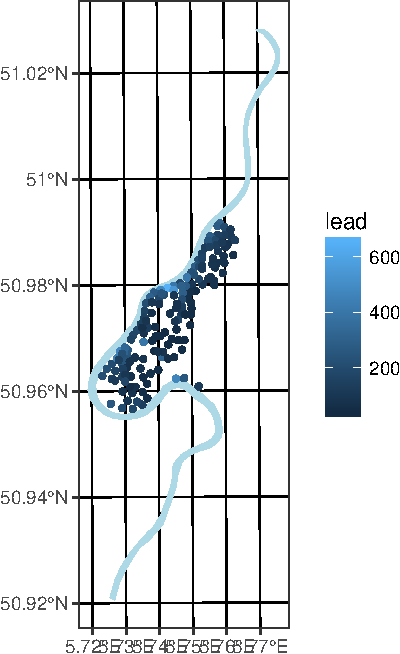
\includegraphics[width=0.33\textwidth]{Lec16_files/figure-beamer/unnamed-chunk-13-1} \end{center}

\end{frame}

\begin{frame}[fragile,t]{ggplot2 - axis limits}
\protect\hypertarget{ggplot2---axis-limits}{}

\scriptoutput

\begin{Shaded}
\begin{Highlighting}[]
\KeywordTok{ggplot}\NormalTok{() }\OperatorTok{+}
\StringTok{  }\KeywordTok{geom_sf}\NormalTok{(}\DataTypeTok{data=}\KeywordTok{st_sf}\NormalTok{(meuse_riv), }\DataTypeTok{fill=}\StringTok{"lightblue"}\NormalTok{, }\DataTypeTok{color=}\OtherTok{NA}\NormalTok{) }\OperatorTok{+}
\StringTok{  }\KeywordTok{geom_sf}\NormalTok{(}\DataTypeTok{data=}\NormalTok{meuse, }\KeywordTok{aes}\NormalTok{(}\DataTypeTok{color=}\NormalTok{lead), }\DataTypeTok{size=}\DecValTok{1}\NormalTok{) }\OperatorTok{+}
\StringTok{  }\KeywordTok{ylim}\NormalTok{(}\FloatTok{50.95}\NormalTok{, }\FloatTok{50.99}\NormalTok{)}
\end{Highlighting}
\end{Shaded}

\begin{center}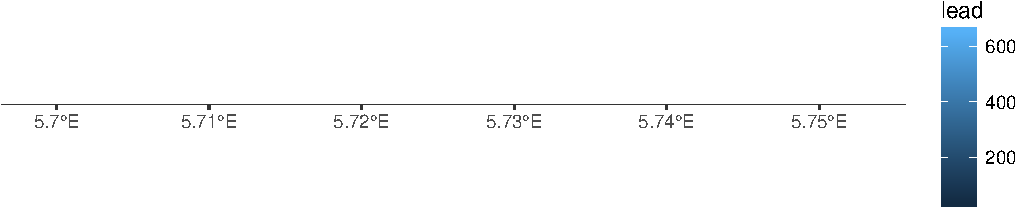
\includegraphics[width=0.65\textwidth]{Lec16_files/figure-beamer/unnamed-chunk-14-1} \end{center}

\end{frame}

\begin{frame}[fragile,t]{ggplot2 - axis limits}
\protect\hypertarget{ggplot2---axis-limits-1}{}

\scriptoutput

\begin{Shaded}
\begin{Highlighting}[]
\KeywordTok{ggplot}\NormalTok{() }\OperatorTok{+}
\StringTok{  }\KeywordTok{geom_sf}\NormalTok{(}\DataTypeTok{data=}\KeywordTok{st_sf}\NormalTok{(meuse_riv), }\DataTypeTok{fill=}\StringTok{"lightblue"}\NormalTok{, }\DataTypeTok{color=}\OtherTok{NA}\NormalTok{) }\OperatorTok{+}
\StringTok{  }\KeywordTok{geom_sf}\NormalTok{(}\DataTypeTok{data=}\NormalTok{meuse, }\KeywordTok{aes}\NormalTok{(}\DataTypeTok{color=}\NormalTok{lead), }\DataTypeTok{size=}\DecValTok{1}\NormalTok{) }\OperatorTok{+}
\StringTok{  }\KeywordTok{ylim}\NormalTok{(}\DecValTok{329714}\NormalTok{, }\DecValTok{333611}\NormalTok{)}
\end{Highlighting}
\end{Shaded}

\begin{center}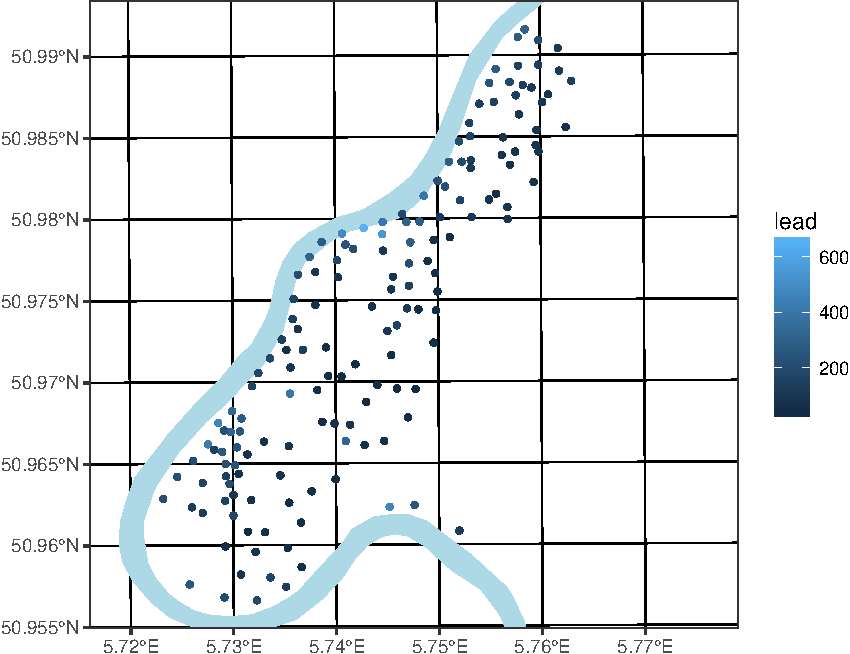
\includegraphics[width=0.65\textwidth]{Lec16_files/figure-beamer/unnamed-chunk-15-1} \end{center}

\end{frame}

\begin{frame}[fragile,t]{ggplot2 - bounding box}
\protect\hypertarget{ggplot2---bounding-box}{}

\scriptoutput

\begin{Shaded}
\begin{Highlighting}[]
\KeywordTok{ggplot}\NormalTok{() }\OperatorTok{+}
\StringTok{  }\KeywordTok{geom_sf}\NormalTok{(}\DataTypeTok{data=}\KeywordTok{st_sf}\NormalTok{(meuse_riv), }\DataTypeTok{fill=}\StringTok{"lightblue"}\NormalTok{, }\DataTypeTok{color=}\OtherTok{NA}\NormalTok{) }\OperatorTok{+}
\StringTok{  }\KeywordTok{geom_sf}\NormalTok{(}\DataTypeTok{data=}\NormalTok{meuse, }\KeywordTok{aes}\NormalTok{(}\DataTypeTok{color=}\NormalTok{lead), }\DataTypeTok{size=}\DecValTok{1}\NormalTok{) }\OperatorTok{+}
\StringTok{  }\KeywordTok{ylim}\NormalTok{(}\KeywordTok{st_bbox}\NormalTok{(meuse)[}\StringTok{"ymin"}\NormalTok{], }\KeywordTok{st_bbox}\NormalTok{(meuse)[}\StringTok{"ymax"}\NormalTok{])}
\end{Highlighting}
\end{Shaded}

\begin{center}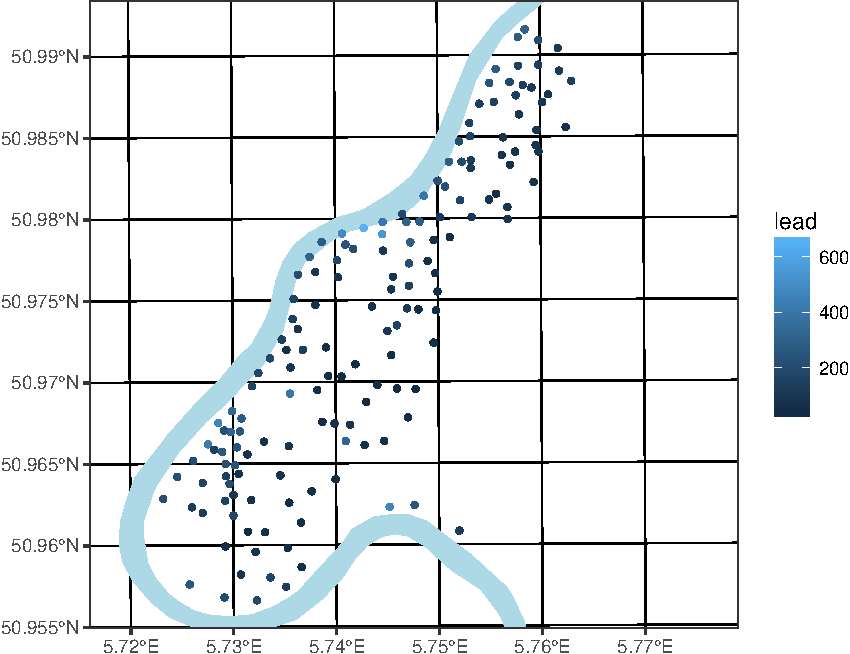
\includegraphics[width=0.65\textwidth]{Lec16_files/figure-beamer/unnamed-chunk-16-1} \end{center}

\end{frame}

\hypertarget{geometry-manipulation}{%
\section{Geometry Manipulation}\label{geometry-manipulation}}

\begin{frame}[fragile,t]{Casting}
\protect\hypertarget{casting}{}

\scriptoutput

\begin{Shaded}
\begin{Highlighting}[]
\NormalTok{nc_pts =}\StringTok{ }\KeywordTok{st_cast}\NormalTok{(nc, }\StringTok{"MULTIPOINT"}\NormalTok{)}

\KeywordTok{tbl_df}\NormalTok{(nc_pts)}
\NormalTok{## # A tibble: 100 x 8}
\NormalTok{##    NAME  BIR74 SID74 NWBIR74 BIR79 SID79 NWBIR79                  geometry}
\NormalTok{##  * <fct> <dbl> <dbl>   <dbl> <dbl> <dbl>   <dbl>          <MULTIPOINT [°]>}
\NormalTok{##  1 Ashe  1091.    1.     10. 1364.    0.     19. (-81.47276 36.23436, -81~}
\NormalTok{##  2 Alle~  487.    0.     10.  542.    3.     12. (-81.23989 36.36536, -81~}
\NormalTok{##  3 Surry 3188.    5.    208. 3616.    6.    260. (-80.45634 36.24256, -80~}
\NormalTok{##  4 Curr~  508.    1.    123.  830.    2.    145. (-76.00897 36.3196, -76.~}
\NormalTok{##  5 Nort~ 1421.    9.   1066. 1606.    3.   1197. (-77.21767 36.24098, -77~}
\NormalTok{##  6 Hert~ 1452.    7.    954. 1838.    5.   1237. (-76.74506 36.23392, -76~}
\NormalTok{##  7 Camd~  286.    0.    115.  350.    2.    139. (-76.00897 36.3196, -75.~}
\NormalTok{##  8 Gates  420.    0.    254.  594.    2.    371. (-76.56251 36.34057, -76~}
\NormalTok{##  9 Warr~  968.    4.    748. 1190.    2.    844. (-78.30876 36.26004, -78~}
\NormalTok{## 10 Stok~ 1612.    1.    160. 2038.    5.    176. (-80.02567 36.25023, -80~}
\NormalTok{## # ... with 90 more rows}
\end{Highlighting}
\end{Shaded}

\end{frame}

\begin{frame}[fragile,t]{}
\protect\hypertarget{section}{}

\scriptoutput

\begin{Shaded}
\begin{Highlighting}[]
\KeywordTok{plot}\NormalTok{(}\KeywordTok{st_geometry}\NormalTok{(nc), }\DataTypeTok{border=}\StringTok{'grey'}\NormalTok{)}
\KeywordTok{plot}\NormalTok{(}\KeywordTok{st_geometry}\NormalTok{(nc_pts), }\DataTypeTok{pch=}\DecValTok{16}\NormalTok{, }\DataTypeTok{cex=}\FloatTok{0.5}\NormalTok{, }\DataTypeTok{add=}\OtherTok{TRUE}\NormalTok{)}
\end{Highlighting}
\end{Shaded}

\begin{center}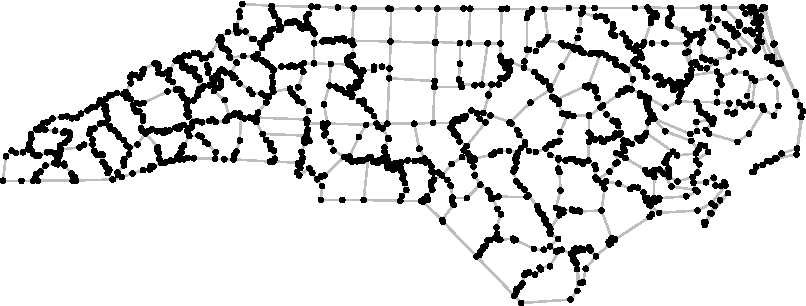
\includegraphics[width=\textwidth]{Lec16_files/figure-beamer/unnamed-chunk-18-1} \end{center}

\end{frame}

\begin{frame}[fragile,t]{Casting - POINT}
\protect\hypertarget{casting---point}{}

\scriptoutput

\begin{Shaded}
\begin{Highlighting}[]
\KeywordTok{st_cast}\NormalTok{(nc, }\StringTok{"POINT"}\NormalTok{)}
\NormalTok{## Simple feature collection with 2529 features and 7 fields}
\NormalTok{## geometry type:  POINT}
\NormalTok{## dimension:      XY}
\NormalTok{## bbox:           xmin: -84.32385 ymin: 33.88199 xmax: -75.45698 ymax: 36.58965}
\NormalTok{## epsg (SRID):    4267}
\NormalTok{## proj4string:    +proj=longlat +datum=NAD27 +no_defs}
\NormalTok{## First 10 features:}
\NormalTok{##    NAME BIR74 SID74 NWBIR74 BIR79 SID79 NWBIR79                   geometry}
\NormalTok{## 1  Ashe  1091     1      10  1364     0      19 POINT (-81.47276 36.23436)}
\NormalTok{## 2  Ashe  1091     1      10  1364     0      19 POINT (-81.54084 36.27251)}
\NormalTok{## 3  Ashe  1091     1      10  1364     0      19 POINT (-81.56198 36.27359)}
\NormalTok{## 4  Ashe  1091     1      10  1364     0      19 POINT (-81.63306 36.34069)}
\NormalTok{## 5  Ashe  1091     1      10  1364     0      19 POINT (-81.74107 36.39178)}
\NormalTok{## 6  Ashe  1091     1      10  1364     0      19 POINT (-81.69828 36.47178)}
\NormalTok{## 7  Ashe  1091     1      10  1364     0      19  POINT (-81.7028 36.51934)}
\NormalTok{## 8  Ashe  1091     1      10  1364     0      19    POINT (-81.67 36.58965)}
\NormalTok{## 9  Ashe  1091     1      10  1364     0      19  POINT (-81.3453 36.57286)}
\NormalTok{## 10 Ashe  1091     1      10  1364     0      19 POINT (-81.34754 36.53791)}
\end{Highlighting}
\end{Shaded}

\end{frame}

\begin{frame}[fragile,t]{}
\protect\hypertarget{section-1}{}

\scriptoutput

\begin{Shaded}
\begin{Highlighting}[]
\KeywordTok{plot}\NormalTok{(}\KeywordTok{st_geometry}\NormalTok{(nc), }\DataTypeTok{border=}\StringTok{'grey'}\NormalTok{)}
\KeywordTok{plot}\NormalTok{(}\KeywordTok{st_geometry}\NormalTok{(}\KeywordTok{st_cast}\NormalTok{(nc, }\StringTok{"POINT"}\NormalTok{)), }\DataTypeTok{pch=}\DecValTok{16}\NormalTok{, }\DataTypeTok{cex=}\FloatTok{0.5}\NormalTok{, }\DataTypeTok{add=}\OtherTok{TRUE}\NormalTok{)}
\end{Highlighting}
\end{Shaded}

\begin{center}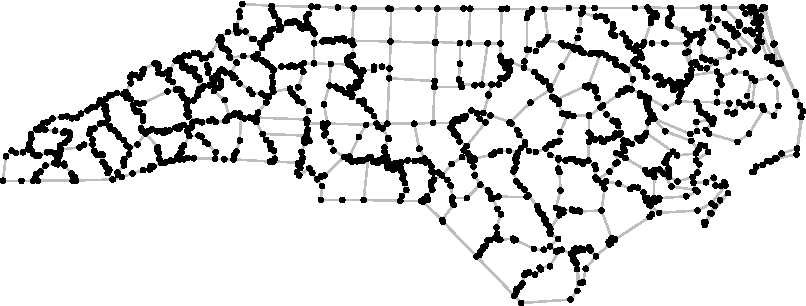
\includegraphics[width=\textwidth]{Lec16_files/figure-beamer/unnamed-chunk-20-1} \end{center}

\end{frame}

\begin{frame}[fragile,t]{Casting - LINESTRING}
\protect\hypertarget{casting---linestring}{}

\scriptoutput

\begin{Shaded}
\begin{Highlighting}[]
\KeywordTok{st_cast}\NormalTok{(nc, }\StringTok{"MULTILINESTRING"}\NormalTok{) }\OperatorTok\StringTok{ }\KeywordTok{as_tibble}\NormalTok{()}
\NormalTok{## # A tibble: 100 x 8}
\NormalTok{##    NAME  BIR74 SID74 NWBIR74 BIR79 SID79 NWBIR79                  geometry}
\NormalTok{##  * <fct> <dbl> <dbl>   <dbl> <dbl> <dbl>   <dbl>     <MULTILINESTRING [°]>}
\NormalTok{##  1 Ashe  1091.    1.     10. 1364.    0.     19. ((-81.47276 36.23436, -8~}
\NormalTok{##  2 Alle~  487.    0.     10.  542.    3.     12. ((-81.23989 36.36536, -8~}
\NormalTok{##  3 Surry 3188.    5.    208. 3616.    6.    260. ((-80.45634 36.24256, -8~}
\NormalTok{##  4 Curr~  508.    1.    123.  830.    2.    145. ((-76.00897 36.3196, -76~}
\NormalTok{##  5 Nort~ 1421.    9.   1066. 1606.    3.   1197. ((-77.21767 36.24098, -7~}
\NormalTok{##  6 Hert~ 1452.    7.    954. 1838.    5.   1237. ((-76.74506 36.23392, -7~}
\NormalTok{##  7 Camd~  286.    0.    115.  350.    2.    139. ((-76.00897 36.3196, -75~}
\NormalTok{##  8 Gates  420.    0.    254.  594.    2.    371. ((-76.56251 36.34057, -7~}
\NormalTok{##  9 Warr~  968.    4.    748. 1190.    2.    844. ((-78.30876 36.26004, -7~}
\NormalTok{## 10 Stok~ 1612.    1.    160. 2038.    5.    176. ((-80.02567 36.25023, -8~}
\NormalTok{## # ... with 90 more rows}
\end{Highlighting}
\end{Shaded}

\end{frame}

\begin{frame}[fragile,t]{}
\protect\hypertarget{section-2}{}

\scriptoutput

\begin{Shaded}
\begin{Highlighting}[]
\KeywordTok{st_cast}\NormalTok{(nc, }\StringTok{"MULTILINESTRING"}\NormalTok{) }\OperatorTok\StringTok{ }\KeywordTok{st_geometry}\NormalTok{() }\OperatorTok\StringTok{ }\KeywordTok{plot}\NormalTok{()}
\end{Highlighting}
\end{Shaded}

\begin{center}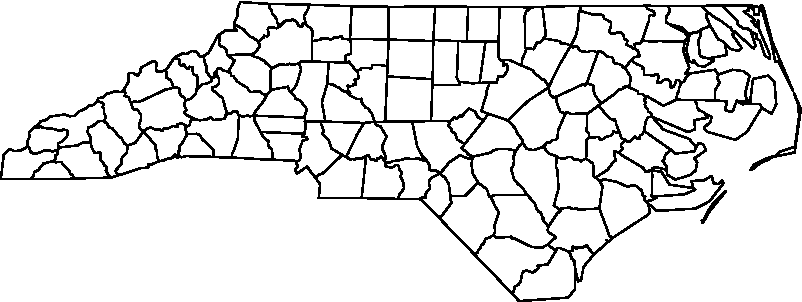
\includegraphics[width=\textwidth]{Lec16_files/figure-beamer/unnamed-chunk-22-1} \end{center}

\end{frame}

\begin{frame}[fragile,t]{Grouping Features}
\protect\hypertarget{grouping-features}{}

\scriptoutput

\begin{Shaded}
\begin{Highlighting}[]
\NormalTok{nc_state =}\StringTok{ }\KeywordTok{st_union}\NormalTok{(nc)}
\KeywordTok{plot}\NormalTok{(nc_state)}
\end{Highlighting}
\end{Shaded}

\begin{center}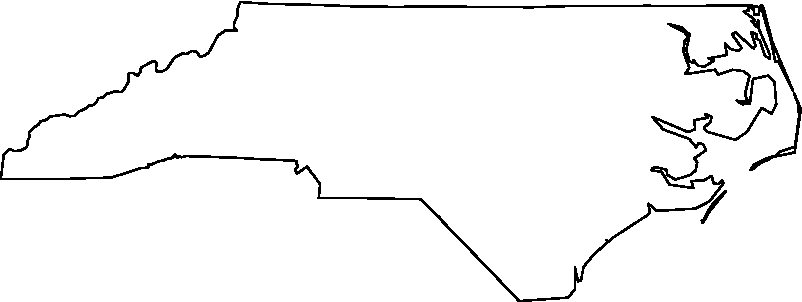
\includegraphics[width=\textwidth]{Lec16_files/figure-beamer/unnamed-chunk-23-1} \end{center}

\begin{Shaded}
\begin{Highlighting}[]

\NormalTok{nc_state}
\NormalTok{## Geometry set for 1 feature }
\NormalTok{## geometry type:  MULTIPOLYGON}
\NormalTok{## dimension:      XY}
\NormalTok{## bbox:           xmin: -84.32385 ymin: 33.88199 xmax: -75.45698 ymax: 36.58965}
\NormalTok{## epsg (SRID):    4267}
\NormalTok{## proj4string:    +proj=longlat +datum=NAD27 +no_defs}
\NormalTok{## MULTIPOLYGON (((-76.54427 34.58783, -76.55515 3...}
\end{Highlighting}
\end{Shaded}

\end{frame}

\begin{frame}[fragile,t]{More Grouping}
\protect\hypertarget{more-grouping}{}

\scriptoutput

\begin{Shaded}
\begin{Highlighting}[]
\NormalTok{nc_cut =}\StringTok{ }\NormalTok{nc }\OperatorTok
\StringTok{  }\KeywordTok{mutate}\NormalTok{(}\DataTypeTok{X =} \KeywordTok{st_centroid}\NormalTok{(nc) }\OperatorTok\StringTok{ }\KeywordTok{st_coordinates}\NormalTok{() }\OperatorTok\StringTok{ }\NormalTok{.[,}\DecValTok{1}\NormalTok{]) }\OperatorTok
\StringTok{  }\KeywordTok{mutate}\NormalTok{(}\DataTypeTok{region =} \KeywordTok{cut}\NormalTok{(X, }\DataTypeTok{breaks =} \DecValTok{5}\NormalTok{))}

\NormalTok{nc_cut}
\NormalTok{## Simple feature collection with 100 features and 9 fields}
\NormalTok{## geometry type:  MULTIPOLYGON}
\NormalTok{## dimension:      XY}
\NormalTok{## bbox:           xmin: -84.32385 ymin: 33.88199 xmax: -75.45698 ymax: 36.58965}
\NormalTok{## epsg (SRID):    4267}
\NormalTok{## proj4string:    +proj=longlat +datum=NAD27 +no_defs}
\NormalTok{## First 10 features:}
\NormalTok{##           NAME BIR74 SID74 NWBIR74 BIR79 SID79 NWBIR79         X}
\NormalTok{## 1         Ashe  1091     1      10  1364     0      19 -81.49826}
\NormalTok{## 2    Alleghany   487     0      10   542     3      12 -81.12515}
\NormalTok{## 3        Surry  3188     5     208  3616     6     260 -80.68575}
\NormalTok{## 4    Currituck   508     1     123   830     2     145 -76.02750}
\NormalTok{## 5  Northampton  1421     9    1066  1606     3    1197 -77.41056}
\NormalTok{## 6     Hertford  1452     7     954  1838     5    1237 -76.99478}
\NormalTok{## 7       Camden   286     0     115   350     2     139 -76.23435}
\NormalTok{## 8        Gates   420     0     254   594     2     371 -76.70448}
\NormalTok{## 9       Warren   968     4     748  1190     2     844 -78.11043}
\NormalTok{## 10      Stokes  1612     1     160  2038     5     176 -80.23428}
\NormalTok{##           region                       geometry}
\NormalTok{## 1  (-82.4,-80.8] MULTIPOLYGON (((-81.47276 3...}
\NormalTok{## 2  (-82.4,-80.8] MULTIPOLYGON (((-81.23989 3...}
\NormalTok{## 3  (-80.8,-79.1] MULTIPOLYGON (((-80.45634 3...}
\NormalTok{## 4  (-77.5,-75.8] MULTIPOLYGON (((-76.00897 3...}
\NormalTok{## 5  (-77.5,-75.8] MULTIPOLYGON (((-77.21767 3...}
\NormalTok{## 6  (-77.5,-75.8] MULTIPOLYGON (((-76.74506 3...}
\NormalTok{## 7  (-77.5,-75.8] MULTIPOLYGON (((-76.00897 3...}
\NormalTok{## 8  (-77.5,-75.8] MULTIPOLYGON (((-76.56251 3...}
\NormalTok{## 9  (-79.1,-77.5] MULTIPOLYGON (((-78.30876 3...}
\NormalTok{## 10 (-80.8,-79.1] MULTIPOLYGON (((-80.02567 3...}
\end{Highlighting}
\end{Shaded}

\end{frame}

\begin{frame}[fragile,t]{}
\protect\hypertarget{section-3}{}

\scriptoutput

\begin{Shaded}
\begin{Highlighting}[]
\KeywordTok{ggplot}\NormalTok{(nc_cut) }\OperatorTok{+}
\StringTok{  }\KeywordTok{geom_sf}\NormalTok{(}\KeywordTok{aes}\NormalTok{(}\DataTypeTok{fill=}\NormalTok{region))}
\end{Highlighting}
\end{Shaded}

\begin{center}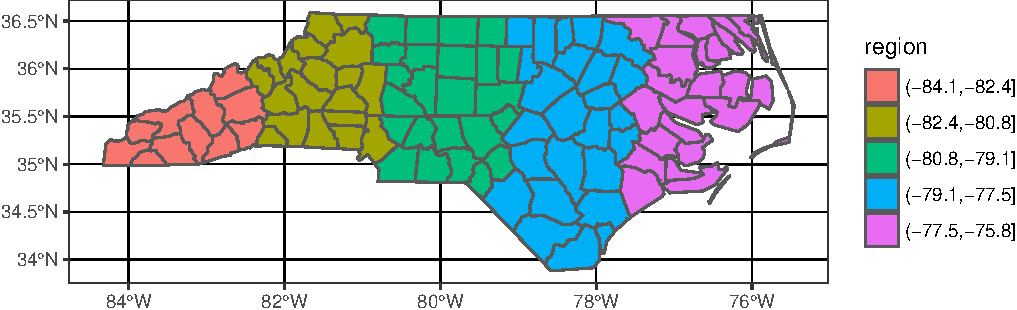
\includegraphics[width=\textwidth]{Lec16_files/figure-beamer/unnamed-chunk-25-1} \end{center}

\end{frame}

\begin{frame}[fragile,t]{dplyr and sf}
\protect\hypertarget{dplyr-and-sf}{}

\scriptoutput

\begin{Shaded}
\begin{Highlighting}[]
\NormalTok{nc_cut }\OperatorTok\StringTok{ }
\StringTok{  }\KeywordTok{group_by}\NormalTok{(region) }\OperatorTok\StringTok{ }
\StringTok{  }\KeywordTok{summarize}\NormalTok{() }\OperatorTok\StringTok{ }
\StringTok{  }\KeywordTok{ggplot}\NormalTok{() }\OperatorTok{+}\StringTok{ }
\StringTok{    }\KeywordTok{geom_sf}\NormalTok{(}\KeywordTok{aes}\NormalTok{(}\DataTypeTok{fill=}\NormalTok{region))}
\end{Highlighting}
\end{Shaded}

\begin{center}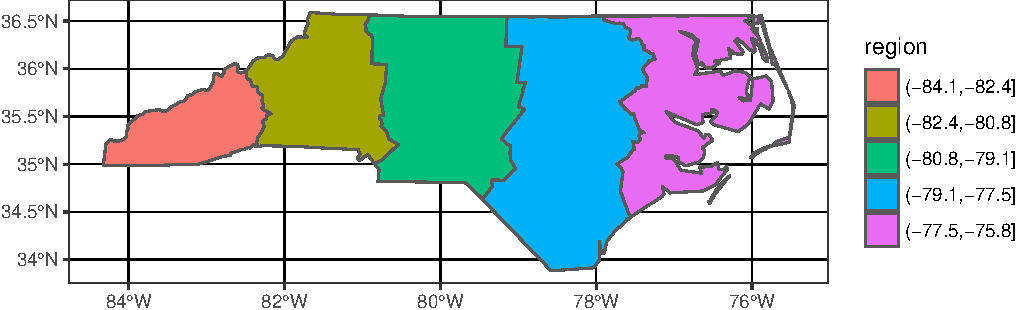
\includegraphics[width=\textwidth]{Lec16_files/figure-beamer/unnamed-chunk-26-1} \end{center}

\end{frame}

\begin{frame}[fragile,t]{Affine Transfomations}
\protect\hypertarget{affine-transfomations}{}

\scriptoutput

\begin{Shaded}
\begin{Highlighting}[]
\NormalTok{rotate =}\StringTok{ }\ControlFlowTok{function}\NormalTok{(a) }\KeywordTok{matrix}\NormalTok{(}\KeywordTok{c}\NormalTok{(}\KeywordTok{cos}\NormalTok{(a), }\KeywordTok{sin}\NormalTok{(a), }\OperatorTok{-}\KeywordTok{sin}\NormalTok{(a), }\KeywordTok{cos}\NormalTok{(a)), }\DecValTok{2}\NormalTok{, }\DecValTok{2}\NormalTok{)}

\NormalTok{ctrd =}\StringTok{ }\KeywordTok{st_centroid}\NormalTok{(nc_state)}
\NormalTok{state_rotate =}\StringTok{ }\NormalTok{lwgeom}\OperatorTok{::}\KeywordTok{st_make_valid}\NormalTok{( (nc_state) }\OperatorTok{*}\StringTok{ }\KeywordTok{rotate}\NormalTok{(}\OperatorTok{-}\NormalTok{pi}\OperatorTok{/}\DecValTok{4}\NormalTok{) )}
\KeywordTok{plot}\NormalTok{(state_rotate, }\DataTypeTok{axes=}\OtherTok{TRUE}\NormalTok{)}
\end{Highlighting}
\end{Shaded}

\begin{center}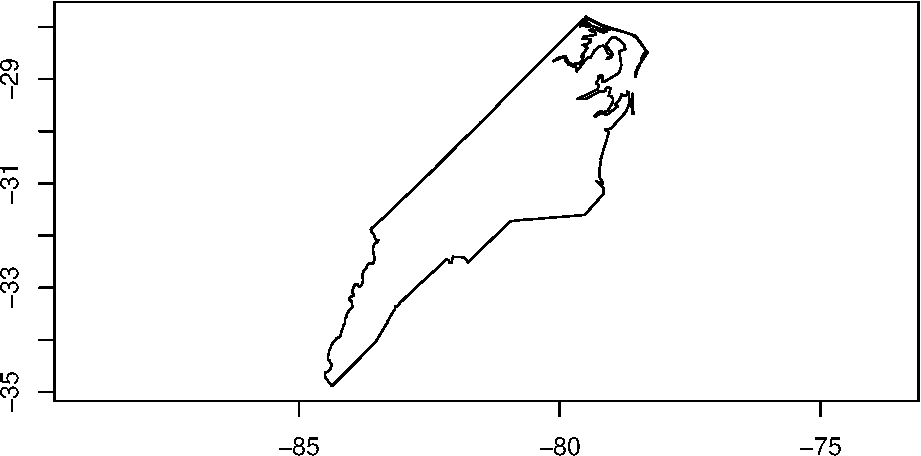
\includegraphics[width=\textwidth]{Lec16_files/figure-beamer/unnamed-chunk-27-1} \end{center}

\end{frame}

\begin{frame}[fragile]{Scaling Size}
\protect\hypertarget{scaling-size}{}

\scriptoutput

\begin{Shaded}
\begin{Highlighting}[]
\NormalTok{ctrd =}\StringTok{ }\KeywordTok{st_centroid}\NormalTok{(}\KeywordTok{st_geometry}\NormalTok{(nc))}
\NormalTok{area =}\StringTok{ }\KeywordTok{st_area}\NormalTok{(nc) }\OperatorTok\StringTok{ }\KeywordTok{strip_attrs}\NormalTok{()}

\NormalTok{nc_rot =}\StringTok{ }\NormalTok{nc}
\KeywordTok{st_geometry}\NormalTok{(nc_rot) =}\StringTok{ }\NormalTok{(}\KeywordTok{st_geometry}\NormalTok{(nc) }\OperatorTok{-}\StringTok{ }\NormalTok{ctrd) }\OperatorTok{*}\StringTok{ }\KeywordTok{rotate}\NormalTok{(pi}\OperatorTok{/}\DecValTok{2}\NormalTok{) }\OperatorTok{*}\StringTok{ }\FloatTok{.5} \OperatorTok{+}\StringTok{ }\NormalTok{ctrd}

\KeywordTok{plot}\NormalTok{(nc_rot[,}\StringTok{"SID79"}\NormalTok{])}
\end{Highlighting}
\end{Shaded}

\begin{center}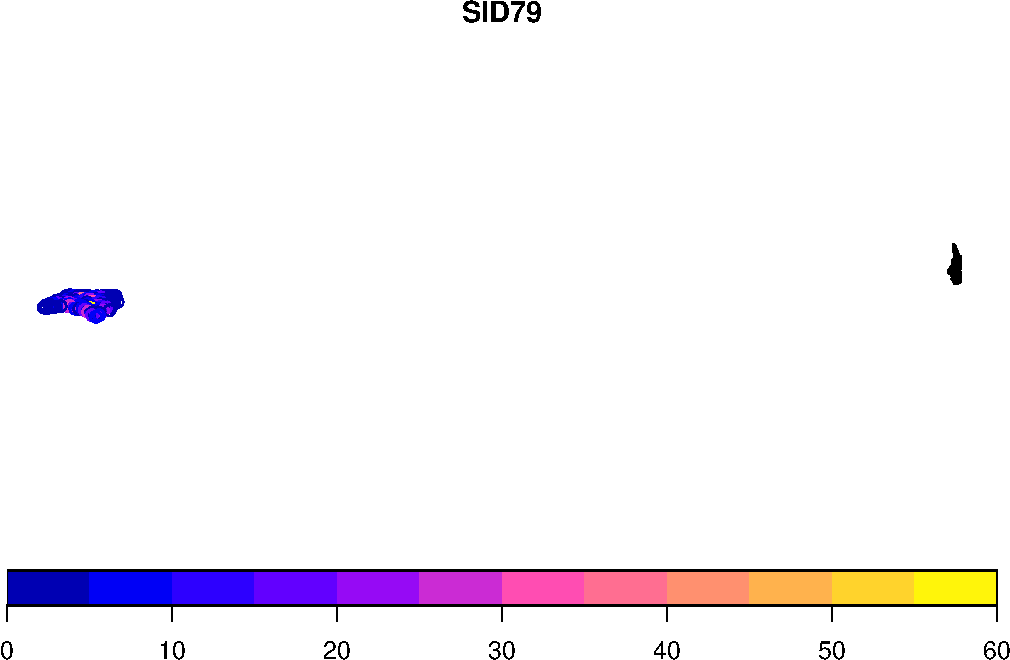
\includegraphics[width=\textwidth]{Lec16_files/figure-beamer/unnamed-chunk-28-1} \end{center}

\end{frame}

\hypertarget{highway-example}{%
\section{Highway Example}\label{highway-example}}

\begin{frame}[fragile,t]{Highways}
\protect\hypertarget{highways}{}

\scriptoutput

\begin{Shaded}
\begin{Highlighting}[]
\NormalTok{hwy =}\StringTok{ }\KeywordTok{st_read}\NormalTok{(}\StringTok{"../data/gis/us_interstates/"}\NormalTok{, }\DataTypeTok{quiet=}\OtherTok{TRUE}\NormalTok{, }\DataTypeTok{stringsAsFactors=}\OtherTok{FALSE}\NormalTok{) }\OperatorTok\StringTok{ }\KeywordTok{st_transform}\NormalTok{(}\KeywordTok{st_crs}\NormalTok{(nc))}

\KeywordTok{ggplot}\NormalTok{() }\OperatorTok{+}
\StringTok{  }\KeywordTok{geom_sf}\NormalTok{(}\DataTypeTok{data=}\NormalTok{nc) }\OperatorTok{+}
\StringTok{  }\KeywordTok{geom_sf}\NormalTok{(}\DataTypeTok{data=}\NormalTok{hwy, }\DataTypeTok{col=}\StringTok{'red'}\NormalTok{)}
\end{Highlighting}
\end{Shaded}

\begin{center}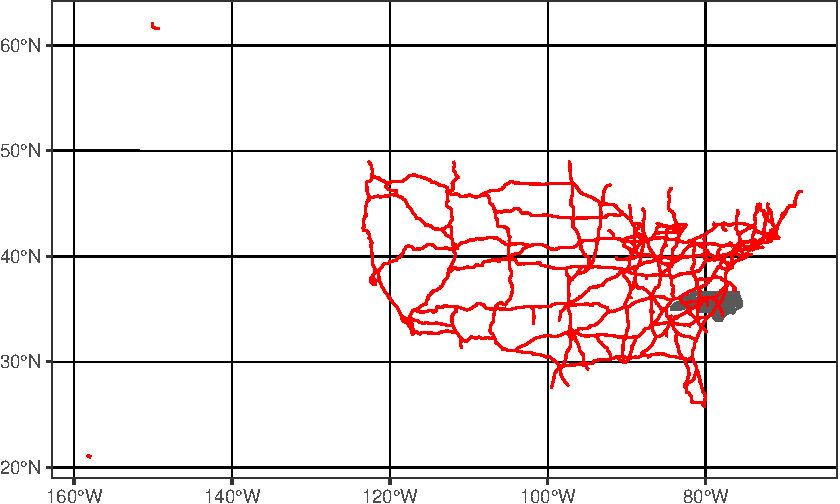
\includegraphics[width=\textwidth]{Lec16_files/figure-beamer/unnamed-chunk-29-1} \end{center}

\end{frame}

\begin{frame}[fragile,t]{NC Interstate Highways}
\protect\hypertarget{nc-interstate-highways}{}

\scriptoutput

\begin{Shaded}
\begin{Highlighting}[]
\NormalTok{hwy_nc =}\StringTok{ }\KeywordTok{st_intersection}\NormalTok{(hwy, nc)}
\NormalTok{## although coordinates are longitude/latitude, st_intersection assumes that they are planar}

\KeywordTok{ggplot}\NormalTok{() }\OperatorTok{+}\StringTok{ }
\StringTok{  }\KeywordTok{geom_sf}\NormalTok{(}\DataTypeTok{data=}\NormalTok{nc) }\OperatorTok{+}
\StringTok{  }\KeywordTok{geom_sf}\NormalTok{(}\DataTypeTok{data=}\NormalTok{hwy_nc, }\DataTypeTok{col=}\StringTok{'red'}\NormalTok{)}
\end{Highlighting}
\end{Shaded}

\begin{center}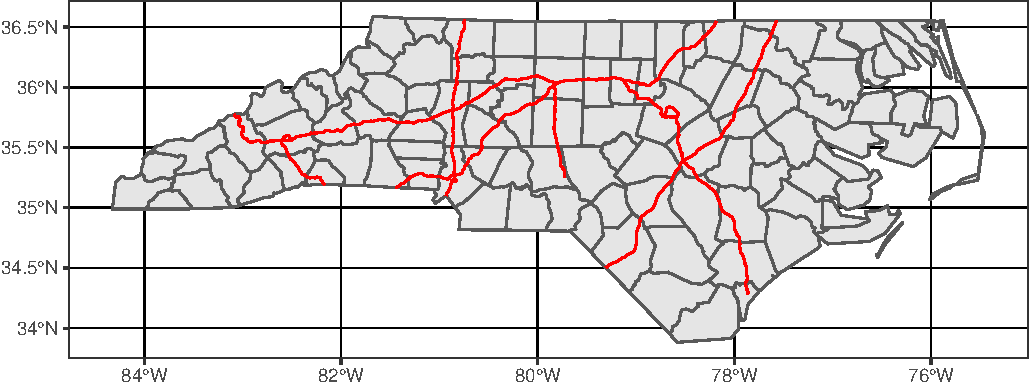
\includegraphics[width=\textwidth]{Lec16_files/figure-beamer/unnamed-chunk-30-1} \end{center}

\end{frame}

\begin{frame}[fragile,t]{Counties near the interstate (Projection)}
\protect\hypertarget{counties-near-the-interstate-projection}{}

\scriptoutput

\begin{Shaded}
\begin{Highlighting}[]
\NormalTok{nc_utm  =}\StringTok{ }\KeywordTok{st_transform}\NormalTok{(nc, }\StringTok{"+proj=utm +zone=17 +datum=NAD83 +units=m +no_defs"}\NormalTok{)}

\KeywordTok{ggplot}\NormalTok{() }\OperatorTok{+}\StringTok{ }
\StringTok{  }\KeywordTok{geom_sf}\NormalTok{(}\DataTypeTok{data=}\NormalTok{nc_utm) }\OperatorTok{+}
\StringTok{  }\KeywordTok{geom_sf}\NormalTok{(}\DataTypeTok{data=}\NormalTok{hwy_nc, }\DataTypeTok{col=}\StringTok{'red'}\NormalTok{)}
\end{Highlighting}
\end{Shaded}

\begin{center}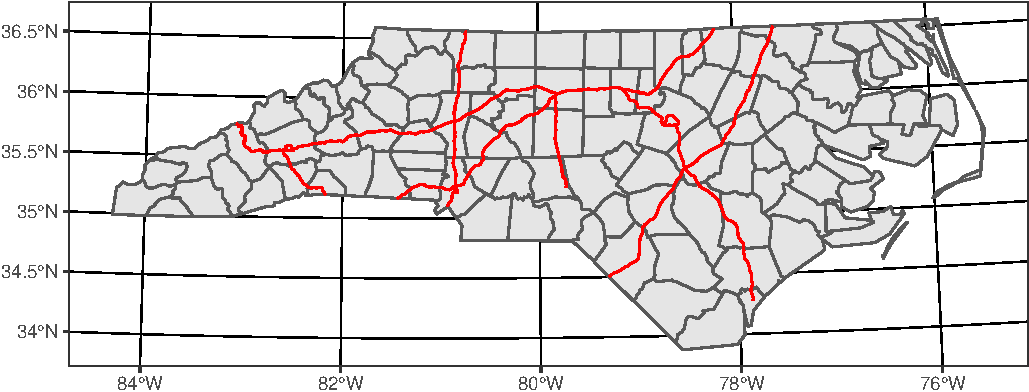
\includegraphics[width=\textwidth]{Lec16_files/figure-beamer/unnamed-chunk-31-1} \end{center}

\end{frame}

\begin{frame}[fragile,t]{Counties near the interstate (Buffering)}
\protect\hypertarget{counties-near-the-interstate-buffering}{}

\scriptoutput

\begin{Shaded}
\begin{Highlighting}[]
\NormalTok{hwy_nc_buffer =}\StringTok{ }\NormalTok{hwy_nc }\OperatorTok
\StringTok{  }\KeywordTok{st_transform}\NormalTok{(}\StringTok{"+proj=utm +zone=17 +datum=NAD83 +units=m +no_defs"}\NormalTok{) }\OperatorTok
\StringTok{  }\KeywordTok{st_buffer}\NormalTok{(}\DecValTok{10000}\NormalTok{)}

\KeywordTok{ggplot}\NormalTok{() }\OperatorTok{+}\StringTok{ }
\StringTok{  }\KeywordTok{geom_sf}\NormalTok{(}\DataTypeTok{data=}\NormalTok{nc_utm) }\OperatorTok{+}
\StringTok{  }\KeywordTok{geom_sf}\NormalTok{(}\DataTypeTok{data=}\NormalTok{hwy_nc, }\DataTypeTok{color=}\StringTok{'red'}\NormalTok{) }\OperatorTok{+}
\StringTok{  }\KeywordTok{geom_sf}\NormalTok{(}\DataTypeTok{data=}\NormalTok{hwy_nc_buffer, }\DataTypeTok{fill=}\StringTok{'red'}\NormalTok{, }\DataTypeTok{alpha=}\FloatTok{0.3}\NormalTok{)}
\end{Highlighting}
\end{Shaded}

\begin{center}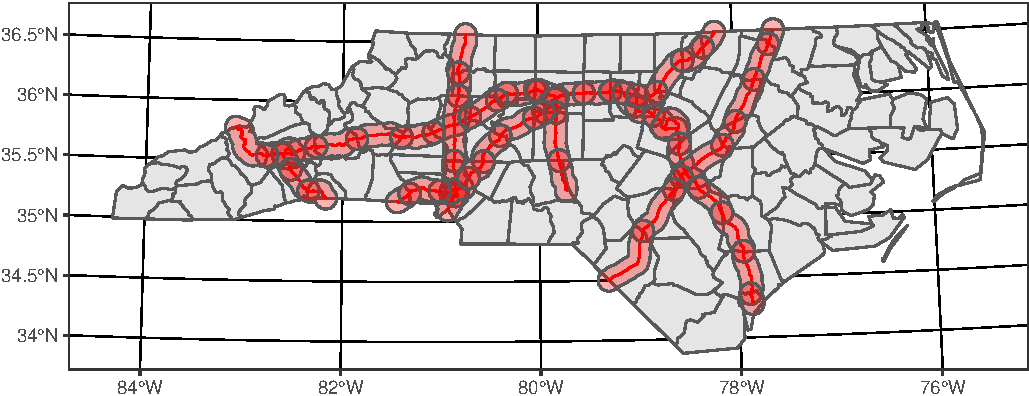
\includegraphics[width=\textwidth]{Lec16_files/figure-beamer/unnamed-chunk-32-1} \end{center}

\end{frame}

\begin{frame}[fragile,t]{Counties near the interstate (Buffering +
Union)}
\protect\hypertarget{counties-near-the-interstate-buffering-union}{}

\scriptoutput

\begin{Shaded}
\begin{Highlighting}[]
\NormalTok{hwy_nc_buffer =}\StringTok{ }\NormalTok{hwy_nc }\OperatorTok
\StringTok{  }\KeywordTok{st_transform}\NormalTok{(}\StringTok{"+proj=utm +zone=17 +datum=NAD83 +units=m +no_defs"}\NormalTok{) }\OperatorTok
\StringTok{  }\KeywordTok{st_buffer}\NormalTok{(}\DecValTok{10000}\NormalTok{) }\OperatorTok
\StringTok{  }\KeywordTok{st_union}\NormalTok{() }\OperatorTok
\StringTok{  }\KeywordTok{st_sf}\NormalTok{()}
  
\KeywordTok{ggplot}\NormalTok{() }\OperatorTok{+}\StringTok{ }
\StringTok{  }\KeywordTok{geom_sf}\NormalTok{(}\DataTypeTok{data=}\NormalTok{nc_utm) }\OperatorTok{+}
\StringTok{  }\KeywordTok{geom_sf}\NormalTok{(}\DataTypeTok{data=}\NormalTok{hwy_nc, }\DataTypeTok{color=}\StringTok{'red'}\NormalTok{) }\OperatorTok{+}
\StringTok{  }\KeywordTok{geom_sf}\NormalTok{(}\DataTypeTok{data=}\NormalTok{hwy_nc_buffer, }\DataTypeTok{fill=}\StringTok{'red'}\NormalTok{, }\DataTypeTok{alpha=}\FloatTok{0.3}\NormalTok{)}
\end{Highlighting}
\end{Shaded}

\begin{center}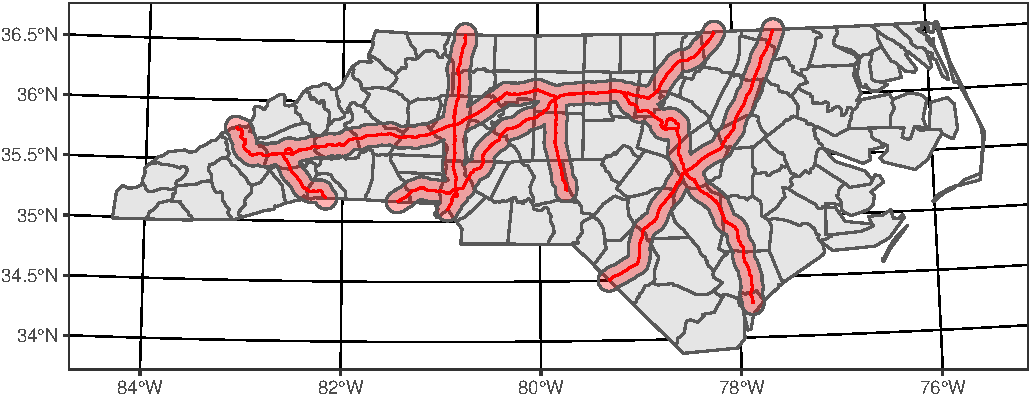
\includegraphics[width=\textwidth]{Lec16_files/figure-beamer/unnamed-chunk-33-1} \end{center}

\end{frame}

\begin{frame}[t]{Example}
\protect\hypertarget{example}{}

How many counties in North Carolina are within 5, 10, 20, or 50 km of an
interstate highway?

\pause

\end{frame}

\hypertarget{gerrymandering-example}{%
\section{Gerrymandering Example}\label{gerrymandering-example}}

\begin{frame}[fragile]{2014 NC House Districts}
\protect\hypertarget{nc-house-districts}{}

\footnoteoutput

\begin{Shaded}
\begin{Highlighting}[]
\NormalTok{nc_house =}\StringTok{ }\KeywordTok{st_read}\NormalTok{(}\StringTok{"../data/nc_districts114.shp"}\NormalTok{, }\DataTypeTok{stringsAsFactors =} \OtherTok{FALSE}\NormalTok{, }\DataTypeTok{quiet =} \OtherTok{TRUE}\NormalTok{) }\OperatorTok
\StringTok{  }\KeywordTok{select}\NormalTok{(ID, DISTRICT)}

\KeywordTok{tbl_df}\NormalTok{(nc_house)}
\NormalTok{## # A tibble: 13 x 3}
\NormalTok{##    ID           DISTRICT                                          geometry}
\NormalTok{##    <chr>        <chr>                                   <MULTIPOLYGON [°]>}
\NormalTok{##  1 037113114002 2        (((-80.05325 35.80178, -80.04671 35.92066, -79.5~}
\NormalTok{##  2 037113114003 3        (((-75.52398 35.77489, -75.50243 35.74291, -75.4~}
\NormalTok{##  3 037113114004 4        (((-79.47249 36.11374, -79.46936 36.12507, -79.4~}
\NormalTok{##  4 037113114001 1        (((-76.68697 36.11117, -76.6848 36.11495, -76.67~}
\NormalTok{##  5 037113114005 5        (((-81.91805 36.2872, -81.90814 36.30201, -81.89~}
\NormalTok{##  6 037113114006 6        (((-80.97462 36.45285, -80.96323 36.45917, -80.9~}
\NormalTok{##  7 037113114007 7        (((-79.37719 34.97479, -79.37112 34.97781, -79.3~}
\NormalTok{##  8 037113114008 8        (((-80.72606 35.21124, -80.7225 35.21661, -80.72~}
\NormalTok{##  9 037113114009 9        (((-81.10803 35.77749, -81.10582 35.7819, -81.10~}
\NormalTok{## 10 037113114010 10       (((-82.6516 35.60073, -82.64091 35.60736, -82.62~}
\NormalTok{## 11 037113114011 11       (((-84.3218 34.98897, -84.29024 35.22557, -84.28~}
\NormalTok{## 12 037113114012 12       (((-80.97461 35.24055, -80.97357 35.24584, -80.9~}
\NormalTok{## 13 037113114013 13       (((-78.87711 35.75273, -78.87338 35.77312, -78.8~}
\end{Highlighting}
\end{Shaded}

\end{frame}

\begin{frame}[fragile]{}
\protect\hypertarget{section-4}{}

\begin{Shaded}
\begin{Highlighting}[]
\NormalTok{nc_house =}\StringTok{ }\NormalTok{nc_house }\OperatorTok
\StringTok{  }\KeywordTok{st_transform}\NormalTok{(}\StringTok{"+proj=utm +zone=17 +datum=NAD83 +units=km +no_defs"}\NormalTok{)}
\KeywordTok{plot}\NormalTok{(nc_house[,}\StringTok{"DISTRICT"}\NormalTok{], }\DataTypeTok{axes=}\OtherTok{TRUE}\NormalTok{)}
\end{Highlighting}
\end{Shaded}

\begin{center}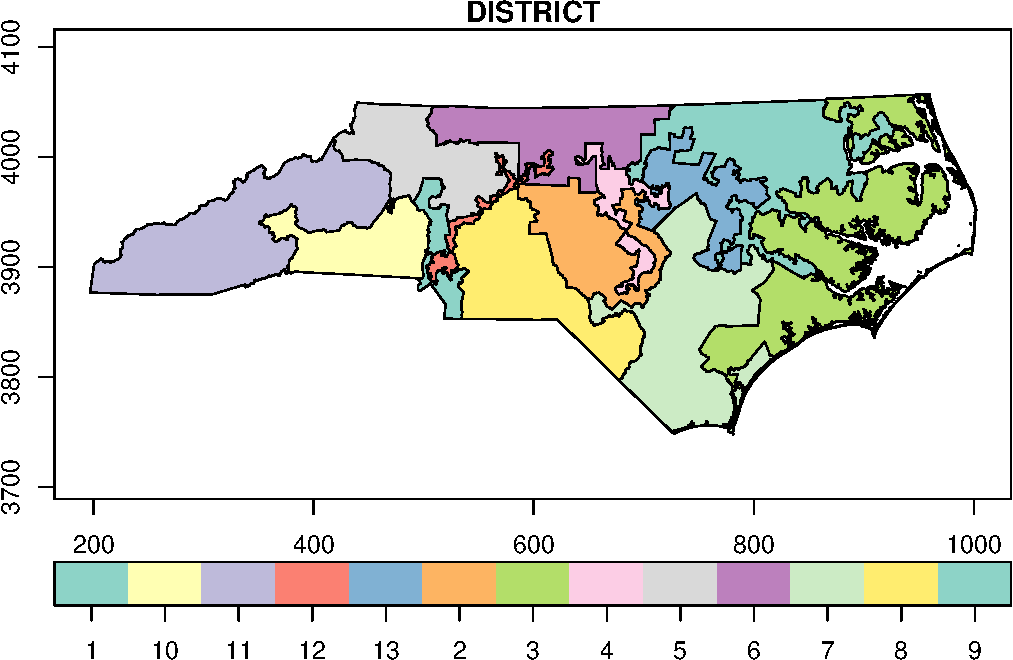
\includegraphics[width=\textwidth]{Lec16_files/figure-beamer/unnamed-chunk-35-1} \end{center}

\end{frame}

\begin{frame}[fragile,t]{Measuring Compactness - Reock Score}
\protect\hypertarget{measuring-compactness---reock-score}{}

The Reock score the a measure of compactness that is calculated as the
the ratio area of a shape to the area of its minimum bounding circle.

\begin{Shaded}
\begin{Highlighting}[]
\NormalTok{circs =}\StringTok{ }\NormalTok{nc_house }\OperatorTok\StringTok{ }\KeywordTok{st_geometry}\NormalTok{() }\OperatorTok\StringTok{ }\NormalTok{lwgeom}\OperatorTok{::}\KeywordTok{st_minimum_bounding_circle}\NormalTok{()}

\NormalTok{sub =}\StringTok{ }\NormalTok{nc_house}\OperatorTok{$}\NormalTok{DISTRICT }\OperatorTok{==}\StringTok{ }\DecValTok{1}
\KeywordTok{plot}\NormalTok{(circs[sub])}
\KeywordTok{plot}\NormalTok{(nc_house[sub,}\StringTok{"DISTRICT"}\NormalTok{], }\DataTypeTok{add=}\OtherTok{TRUE}\NormalTok{)}
\end{Highlighting}
\end{Shaded}

\begin{center}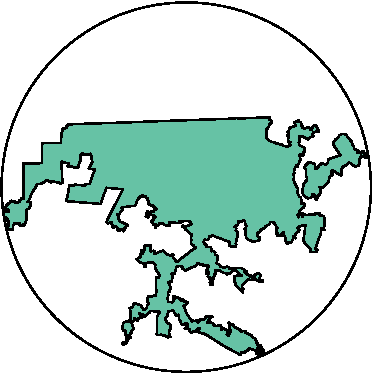
\includegraphics[width=0.4\textwidth]{Lec16_files/figure-beamer/unnamed-chunk-36-1} \end{center}

\end{frame}

\begin{frame}[fragile]{}
\protect\hypertarget{section-5}{}

\begin{Shaded}
\begin{Highlighting}[]
\KeywordTok{plot}\NormalTok{(nc_house[,}\StringTok{"DISTRICT"}\NormalTok{])}
\KeywordTok{plot}\NormalTok{(circs,}\DataTypeTok{add=}\OtherTok{TRUE}\NormalTok{)}
\end{Highlighting}
\end{Shaded}

\begin{center}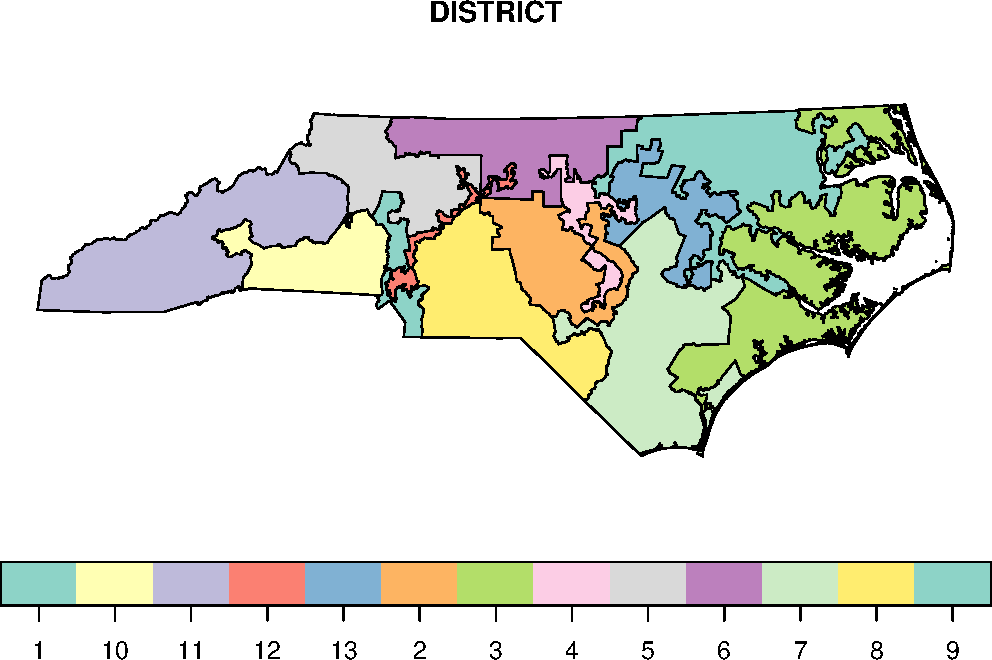
\includegraphics[width=\textwidth]{Lec16_files/figure-beamer/unnamed-chunk-37-1} \end{center}

\end{frame}

\begin{frame}[fragile]{Calculating Reock}
\protect\hypertarget{calculating-reock}{}

\begin{Shaded}
\begin{Highlighting}[]
\NormalTok{nc_house =}\StringTok{ }\NormalTok{nc_house }\OperatorTok
\StringTok{  }\KeywordTok{mutate}\NormalTok{(}\DataTypeTok{reock =} \KeywordTok{st_area}\NormalTok{(nc_house) }\OperatorTok{/}\StringTok{ }\KeywordTok{st_area}\NormalTok{(circs))}
\KeywordTok{plot}\NormalTok{(nc_house[,}\StringTok{"reock"}\NormalTok{])}
\end{Highlighting}
\end{Shaded}

\begin{center}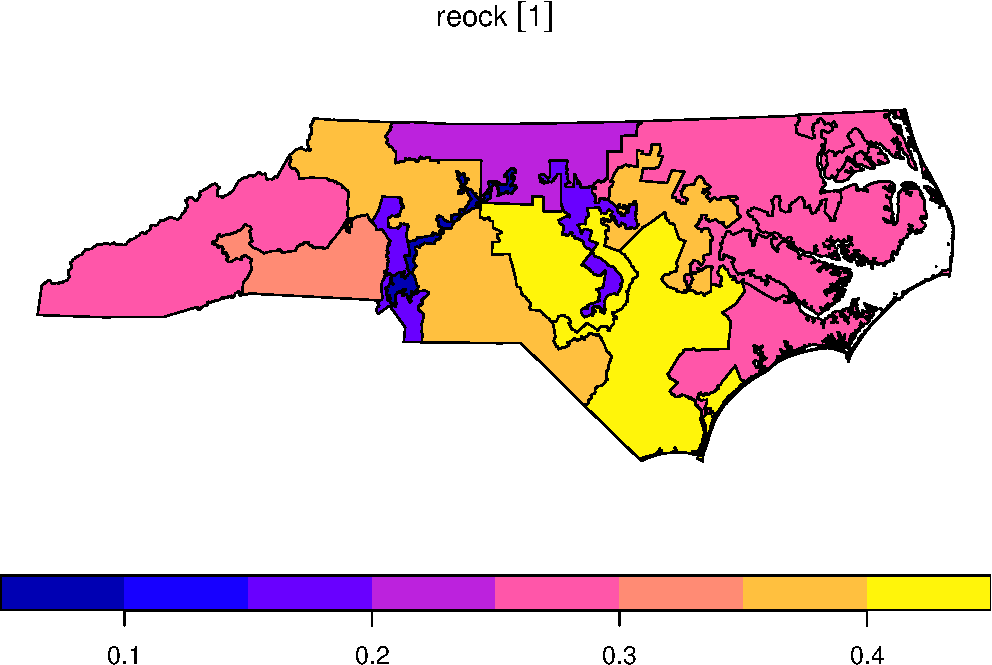
\includegraphics[width=0.8\textwidth]{Lec16_files/figure-beamer/unnamed-chunk-38-1} \end{center}

\end{frame}

\begin{frame}[fragile]{}
\protect\hypertarget{section-6}{}

\begin{Shaded}
\begin{Highlighting}[]
\KeywordTok{tbl_df}\NormalTok{(nc_house) }\OperatorTok\StringTok{ }
\StringTok{  }\KeywordTok{arrange}\NormalTok{(reock) }\OperatorTok
\StringTok{  }\KeywordTok{print}\NormalTok{(}\DataTypeTok{n=}\DecValTok{13}\NormalTok{)}
\NormalTok{## # A tibble: 13 x 4}
\NormalTok{##    ID           DISTRICT reock                                    geometry}
\NormalTok{##    <chr>        <chr>    <S3: units>                   <MULTIPOLYGON [km]>}
\NormalTok{##  1 037113114012 12       0.0711997215878126 (((502.31 3899.72, 502.4045 3~}
\NormalTok{##  2 037113114009 9        0.169405525617443  (((490.2361 3959.275, 490.436~}
\NormalTok{##  3 037113114004 4        0.1735809490213    (((637.4776 3997.644, 637.739~}
\NormalTok{##  4 037113114006 6        0.240919191926239  (((502.2744 4034.178, 503.294~}
\NormalTok{##  5 037113114003 3        0.251285019523225  (((995.1797 3972.839, 997.330~}
\NormalTok{##  6 037113114011 11       0.264255107593438  (((196.7812 3876.863, 200.530~}
\NormalTok{##  7 037113114001 1        0.289934134507595  (((888.2895 4004.901, 888.466~}
\NormalTok{##  8 037113114010 10       0.34012606752961   (((350.3919 3940.92, 351.3727~}
\NormalTok{##  9 037113114008 8        0.353232490504049  (((524.9335 3896.503, 525.255~}
\NormalTok{## 10 037113114013 13       0.382195549931454  (((691.9403 3958.602, 692.228~}
\NormalTok{## 11 037113114005 5        0.397082589710882  (((417.5582 4016.195, 418.464~}
\NormalTok{## 12 037113114007 7        0.414888641986656  (((648.136 3871.45, 648.6853 ~}
\NormalTok{## 13 037113114002 2        0.42590009492903   (((585.5425 3962.377, 586.005~}
\end{Highlighting}
\end{Shaded}

\end{frame}

\hypertarget{raster-data}{%
\section{Raster Data}\label{raster-data}}

\begin{frame}[fragile,t]{Example data - Meuse}
\protect\hypertarget{example-data---meuse-1}{}

\scriptoutput

\begin{Shaded}
\begin{Highlighting}[]
\NormalTok{meuse_rast =}\StringTok{ }\KeywordTok{raster}\NormalTok{(}\KeywordTok{system.file}\NormalTok{(}\StringTok{"external/test.grd"}\NormalTok{, }\DataTypeTok{package=}\StringTok{"raster"}\NormalTok{))}

\NormalTok{meuse_rast}
\NormalTok{## class       : RasterLayer }
\NormalTok{## dimensions  : 115, 80, 9200  (nrow, ncol, ncell)}
\NormalTok{## resolution  : 40, 40  (x, y)}
\NormalTok{## extent      : 178400, 181600, 329400, 334000  (xmin, xmax, ymin, ymax)}
\NormalTok{## coord. ref. : +init=epsg:28992 +towgs84=565.237,50.0087,465.658,-0.406857,0.350733,-1.87035,4.0812 +proj=sterea +lat_0=52.15616055555555 +lon_0=5.38763888888889 +k=0.9999079 +x_0=155000 +y_0=463000 +ellps=bessel +units=m +no_defs }
\NormalTok{## data source : /usr/local/lib/R/3.4/site-library/raster/external/test.grd }
\NormalTok{## names       : test }
\NormalTok{## values      : 128.434, 1805.78  (min, max)}
\end{Highlighting}
\end{Shaded}

\end{frame}

\begin{frame}[fragile,t]{}
\protect\hypertarget{section-7}{}

\scriptoutput

\begin{Shaded}
\begin{Highlighting}[]
\KeywordTok{plot}\NormalTok{(meuse_rast)}
\KeywordTok{plot}\NormalTok{(meuse_riv, }\DataTypeTok{add=}\OtherTok{TRUE}\NormalTok{, }\DataTypeTok{col=}\KeywordTok{adjustcolor}\NormalTok{(}\StringTok{"lightblue"}\NormalTok{,}\DataTypeTok{alpha.f =} \FloatTok{0.5}\NormalTok{), }\DataTypeTok{border=}\OtherTok{NA}\NormalTok{)}
\end{Highlighting}
\end{Shaded}

\begin{center}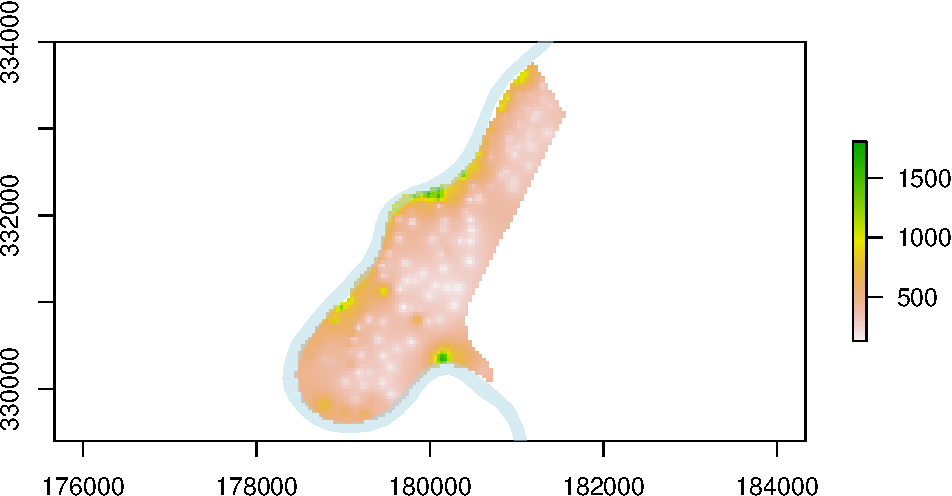
\includegraphics[width=\textwidth]{Lec16_files/figure-beamer/unnamed-chunk-41-1} \end{center}

\end{frame}

\begin{frame}[fragile]{raster class}
\protect\hypertarget{raster-class}{}

\scriptoutput

\begin{Shaded}
\begin{Highlighting}[]
\KeywordTok{str}\NormalTok{(meuse_rast)}
\NormalTok{## Formal class 'RasterLayer' [package "raster"] with 12 slots}
\NormalTok{##   ..@ file    :Formal class '.RasterFile' [package "raster"] with 13 slots}
\NormalTok{##   .. .. ..@ name        : chr "/usr/local/lib/R/3.4/site-library/raster/external/test.grd"}
\NormalTok{##   .. .. ..@ datanotation: chr "FLT4S"}
\NormalTok{##   .. .. ..@ byteorder   : Named chr "little"}
\NormalTok{##   .. .. .. ..- attr(*, "names")= chr "value"}
\NormalTok{##   .. .. ..@ nodatavalue : num -3.4e+38}
\NormalTok{##   .. .. ..@ NAchanged   : logi FALSE}
\NormalTok{##   .. .. ..@ nbands      : int 1}
\NormalTok{##   .. .. ..@ bandorder   : Named chr "BIL"}
\NormalTok{##   .. .. .. ..- attr(*, "names")= chr "value"}
\NormalTok{##   .. .. ..@ offset      : int 0}
\NormalTok{##   .. .. ..@ toptobottom : logi TRUE}
\NormalTok{##   .. .. ..@ blockrows   : int 0}
\NormalTok{##   .. .. ..@ blockcols   : int 0}
\NormalTok{##   .. .. ..@ driver      : chr "raster"}
\NormalTok{##   .. .. ..@ open        : logi FALSE}
\NormalTok{##   ..@ data    :Formal class '.SingleLayerData' [package "raster"] with 13 slots}
\NormalTok{##   .. .. ..@ values    : logi(0) }
\NormalTok{##   .. .. ..@ offset    : num 0}
\NormalTok{##   .. .. ..@ gain      : num 1}
\NormalTok{##   .. .. ..@ inmemory  : logi FALSE}
\NormalTok{##   .. .. ..@ fromdisk  : logi TRUE}
\NormalTok{##   .. .. ..@ isfactor  : logi FALSE}
\NormalTok{##   .. .. ..@ attributes: list()}
\NormalTok{##   .. .. ..@ haveminmax: logi TRUE}
\NormalTok{##   .. .. ..@ min       : num 128}
\NormalTok{##   .. .. ..@ max       : num 1806}
\NormalTok{##   .. .. ..@ band      : int 1}
\NormalTok{##   .. .. ..@ unit      : chr ""}
\NormalTok{##   .. .. ..@ names     : chr "test"}
\NormalTok{##   ..@ legend  :Formal class '.RasterLegend' [package "raster"] with 5 slots}
\NormalTok{##   .. .. ..@ type      : chr(0) }
\NormalTok{##   .. .. ..@ values    : logi(0) }
\NormalTok{##   .. .. ..@ color     : logi(0) }
\NormalTok{##   .. .. ..@ names     : logi(0) }
\NormalTok{##   .. .. ..@ colortable: logi(0) }
\NormalTok{##   ..@ title   : chr(0) }
\NormalTok{##   ..@ extent  :Formal class 'Extent' [package "raster"] with 4 slots}
\NormalTok{##   .. .. ..@ xmin: num 178400}
\NormalTok{##   .. .. ..@ xmax: num 181600}
\NormalTok{##   .. .. ..@ ymin: num 329400}
\NormalTok{##   .. .. ..@ ymax: num 334000}
\NormalTok{##   ..@ rotated : logi FALSE}
\NormalTok{##   ..@ rotation:Formal class '.Rotation' [package "raster"] with 2 slots}
\NormalTok{##   .. .. ..@ geotrans: num(0) }
\NormalTok{##   .. .. ..@ transfun:function ()  }
\NormalTok{##   ..@ ncols   : int 80}
\NormalTok{##   ..@ nrows   : int 115}
\NormalTok{##   ..@ crs     :Formal class 'CRS' [package "sp"] with 1 slot}
\NormalTok{##   .. .. ..@ projargs: chr "+init=epsg:28992 +towgs84=565.237,50.0087,465.658,-0.406857,0.350733,-1.87035,4.0812 +proj=sterea +lat_0=52.156"| __truncated__}
\NormalTok{##   ..@ history : list()}
\NormalTok{##   ..@ z       : list()}
\end{Highlighting}
\end{Shaded}

\end{frame}

\begin{frame}[fragile,t]{raster features}
\protect\hypertarget{raster-features}{}

\scriptoutput

\begin{Shaded}
\begin{Highlighting}[]
\KeywordTok{extent}\NormalTok{(meuse_rast)}
\NormalTok{## class       : Extent }
\NormalTok{## xmin        : 178400 }
\NormalTok{## xmax        : 181600 }
\NormalTok{## ymin        : 329400 }
\NormalTok{## ymax        : 334000}

\KeywordTok{dim}\NormalTok{(meuse_rast)}
\NormalTok{## [1] 115  80   1}

\KeywordTok{res}\NormalTok{(meuse_rast)}
\NormalTok{## [1] 40 40}

\KeywordTok{projection}\NormalTok{(meuse_rast)}
\NormalTok{## [1] "+init=epsg:28992 +towgs84=565.237,50.0087,465.658,-0.406857,0.350733,-1.87035,4.0812 +proj=sterea +lat_0=52.15616055555555 +lon_0=5.38763888888889 +k=0.9999079 +x_0=155000 +y_0=463000 +ellps=bessel +units=m +no_defs"}

\NormalTok{meuse_rast[}\DecValTok{20}\NormalTok{,]}
\NormalTok{##  [1]      NA      NA      NA      NA      NA      NA      NA      NA}
\NormalTok{##  [9]      NA      NA      NA      NA      NA      NA      NA      NA}
\NormalTok{## [17]      NA      NA      NA      NA      NA      NA      NA      NA}
\NormalTok{## [25]      NA      NA      NA      NA      NA      NA      NA      NA}
\NormalTok{## [33]      NA      NA      NA      NA      NA      NA      NA      NA}
\NormalTok{## [41]      NA      NA      NA      NA      NA      NA      NA      NA}
\NormalTok{## [49]      NA      NA      NA      NA      NA      NA      NA      NA}
\NormalTok{## [57]      NA      NA      NA 749.536 895.292 791.145 607.186 511.044}
\NormalTok{## [65] 468.404 399.325 350.362 306.180 300.483 310.082 283.940 285.771}
\NormalTok{## [73] 304.709 309.690 301.799 308.753 328.357 345.611      NA      NA}
\end{Highlighting}
\end{Shaded}

\end{frame}

\begin{frame}[fragile,t]{Rasters and Projections}
\protect\hypertarget{rasters-and-projections}{}

\scriptoutput

\begin{Shaded}
\begin{Highlighting}[]
\KeywordTok{library}\NormalTok{(rgdal)}
\NormalTok{meuse_rast_ll =}\StringTok{ }\KeywordTok{projectRaster}\NormalTok{(meuse_rast, }\DataTypeTok{crs=}\StringTok{"+proj=longlat +datum=NAD27 +no_defs"}\NormalTok{)}

\KeywordTok{par}\NormalTok{(}\DataTypeTok{mfrow=}\KeywordTok{c}\NormalTok{(}\DecValTok{1}\NormalTok{,}\DecValTok{2}\NormalTok{))}
\KeywordTok{plot}\NormalTok{(meuse_rast)}
\KeywordTok{plot}\NormalTok{(meuse_rast_ll)}
\end{Highlighting}
\end{Shaded}

\begin{center}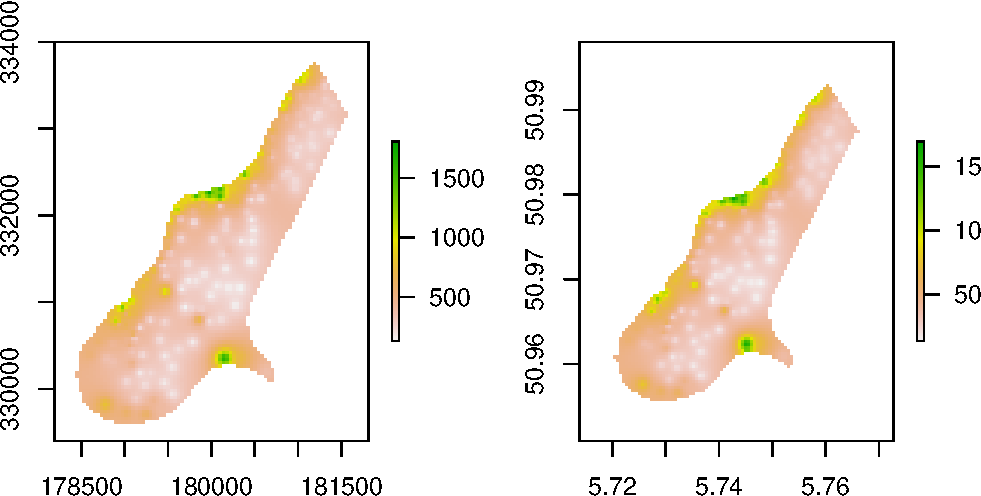
\includegraphics[width=\textwidth]{Lec16_files/figure-beamer/unnamed-chunk-44-1} \end{center}

\end{frame}

\begin{frame}[fragile,t]{}
\protect\hypertarget{section-8}{}

\scriptsize

\begin{Shaded}
\begin{Highlighting}[]
\NormalTok{meuse_rast}
\NormalTok{## class       : RasterLayer }
\NormalTok{## dimensions  : 115, 80, 9200  (nrow, ncol, ncell)}
\NormalTok{## resolution  : 40, 40  (x, y)}
\NormalTok{## extent      : 178400, 181600, 329400, 334000  (xmin, xmax, ymin, ymax)}
\NormalTok{## coord. ref. : +init=epsg:28992 +towgs84=565.237,50.0087,465.658,-0.406857,0.350733,-1.87035,4.0812 +proj=sterea +lat_0=52.15616055555555 +lon_0=5.38763888888889 +k=0.9999079 +x_0=155000 +y_0=463000 +ellps=bessel +units=m +no_defs }
\NormalTok{## data source : /usr/local/lib/R/3.4/site-library/raster/external/test.grd }
\NormalTok{## names       : test }
\NormalTok{## values      : 128.434, 1805.78  (min, max)}

\NormalTok{meuse_rast_ll}
\NormalTok{## class       : RasterLayer }
\NormalTok{## dimensions  : 131, 91, 11921  (nrow, ncol, ncell)}
\NormalTok{## resolution  : 0.000569, 0.00036  (x, y)}
\NormalTok{## extent      : 5.717362, 5.769141, 50.95089, 50.99805  (xmin, xmax, ymin, ymax)}
\NormalTok{## coord. ref. : +proj=longlat +datum=NAD27 +no_defs +ellps=clrk66 +nadgrids=@conus,@alaska,@ntv2_0.gsb,@ntv1_can.dat }
\NormalTok{## data source : in memory}
\NormalTok{## names       : test }
\NormalTok{## values      : 135.647, 1693.578  (min, max)}
\end{Highlighting}
\end{Shaded}

\end{frame}

\begin{frame}[fragile,t]{Simple Features \(\longleftrightarrow\)
Rasters}
\protect\hypertarget{simple-features-longleftrightarrow-rasters}{}

\scriptoutput

\begin{Shaded}
\begin{Highlighting}[]
\NormalTok{meuse_riv_rast =}\StringTok{ }\KeywordTok{rasterize}\NormalTok{(meuse_riv, meuse_rast)}
\NormalTok{## Error in (function (classes, fdef, mtable) : unable to find an inherited method for function 'rasterize' for signature '"sfc_POLYGON", "RasterLayer"'}

\NormalTok{meuse_riv_rast =}\StringTok{ }\KeywordTok{rasterize}\NormalTok{(}\KeywordTok{as}\NormalTok{(meuse_riv, }\StringTok{"Spatial"}\NormalTok{), meuse_rast)}
\KeywordTok{plot}\NormalTok{(meuse_riv_rast)}
\end{Highlighting}
\end{Shaded}

\begin{center}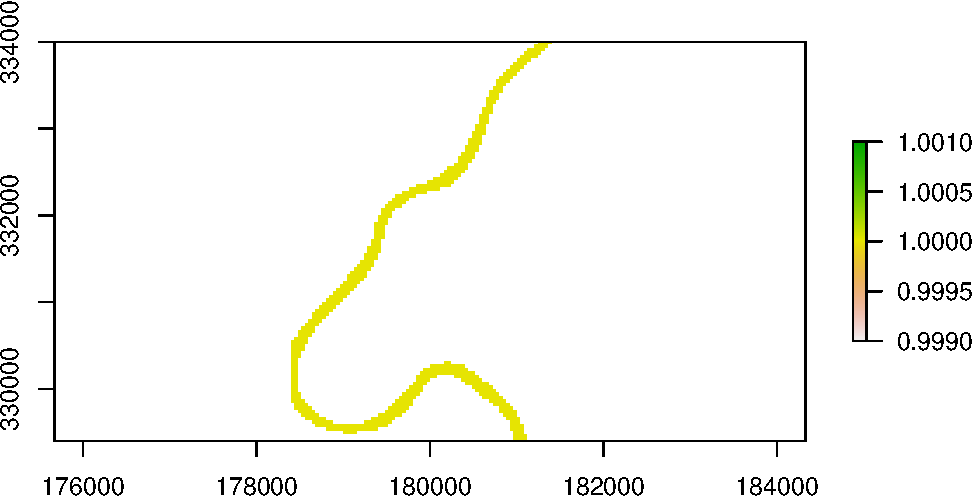
\includegraphics[width=\textwidth]{Lec16_files/figure-beamer/unnamed-chunk-46-1} \end{center}

\end{frame}

\begin{frame}[fragile,t]{Rasters and Spatial Models}
\protect\hypertarget{rasters-and-spatial-models}{}

\scriptoutput

\begin{Shaded}
\begin{Highlighting}[]
\KeywordTok{head}\NormalTok{(meuse)}
\NormalTok{## Simple feature collection with 6 features and 12 fields}
\NormalTok{## geometry type:  POINT}
\NormalTok{## dimension:      XY}
\NormalTok{## bbox:           xmin: 181025 ymin: 333260 xmax: 181390 ymax: 333611}
\NormalTok{## epsg (SRID):    28992}
\NormalTok{## proj4string:    +proj=sterea +lat_0=52.15616055555555 +lon_0=5.38763888888889 +k=0.9999079 +x_0=155000 +y_0=463000 +ellps=bessel +towgs84=565.2369,50.0087,465.658,-0.406857,0.350733,-1.87035,4.0812 +units=m +no_defs}
\NormalTok{##   cadmium copper lead zinc  elev       dist   om ffreq soil lime landuse}
\NormalTok{## 1    11.7     85  299 1022 7.909 0.00135803 13.6     1    1    1      Ah}
\NormalTok{## 2     8.6     81  277 1141 6.983 0.01222430 14.0     1    1    1      Ah}
\NormalTok{## 3     6.5     68  199  640 7.800 0.10302900 13.0     1    1    1      Ah}
\NormalTok{## 4     2.6     81  116  257 7.655 0.19009400  8.0     1    2    0      Ga}
\NormalTok{## 5     2.8     48  117  269 7.480 0.27709000  8.7     1    2    0      Ah}
\NormalTok{## 6     3.0     61  137  281 7.791 0.36406700  7.8     1    2    0      Ga}
\NormalTok{##   dist.m              geometry}
\NormalTok{## 1     50 POINT (181072 333611)}
\NormalTok{## 2     30 POINT (181025 333558)}
\NormalTok{## 3    150 POINT (181165 333537)}
\NormalTok{## 4    270 POINT (181298 333484)}
\NormalTok{## 5    380 POINT (181307 333330)}
\NormalTok{## 6    470 POINT (181390 333260)}

\KeywordTok{head}\NormalTok{(}\KeywordTok{st_coordinates}\NormalTok{(meuse))}
\NormalTok{##        X      Y}
\NormalTok{## 1 181072 333611}
\NormalTok{## 2 181025 333558}
\NormalTok{## 3 181165 333537}
\NormalTok{## 4 181298 333484}
\NormalTok{## 5 181307 333330}
\NormalTok{## 6 181390 333260}
\end{Highlighting}
\end{Shaded}

\end{frame}

\begin{frame}[fragile,t]{}
\protect\hypertarget{section-9}{}

\scriptoutput

\begin{Shaded}
\begin{Highlighting}[]
\KeywordTok{library}\NormalTok{(fields)}

\NormalTok{tps =}\StringTok{ }\KeywordTok{Tps}\NormalTok{(}\DataTypeTok{x =} \KeywordTok{st_coordinates}\NormalTok{(meuse), }\DataTypeTok{Y=}\NormalTok{meuse}\OperatorTok{$}\NormalTok{elev)}
\NormalTok{pred_grid =}\StringTok{ }\KeywordTok{xyFromCell}\NormalTok{(meuse_rast, }\KeywordTok{seq_along}\NormalTok{(meuse_rast))}

\NormalTok{meuse_elev_pred =}\StringTok{ }\NormalTok{meuse_rast}
\NormalTok{meuse_elev_pred[] =}\StringTok{ }\KeywordTok{predict}\NormalTok{(tps, pred_grid)}

\KeywordTok{plot}\NormalTok{(meuse_elev_pred)}
\end{Highlighting}
\end{Shaded}

\begin{center}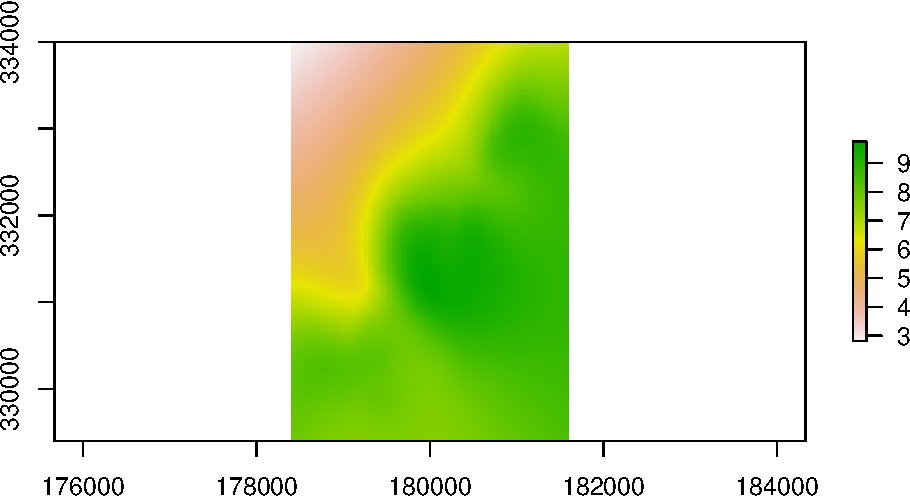
\includegraphics[width=\textwidth]{Lec16_files/figure-beamer/unnamed-chunk-48-1} \end{center}

\end{frame}

\begin{frame}[fragile]{ggplot and rasters}
\protect\hypertarget{ggplot-and-rasters}{}

\begin{Shaded}
\begin{Highlighting}[]
\NormalTok{p =}\StringTok{ }\KeywordTok{rasterToPolygons}\NormalTok{(meuse_elev_pred) }\OperatorTok\StringTok{ }\KeywordTok{st_as_sf}\NormalTok{()}

\NormalTok{(}\KeywordTok{ggplot}\NormalTok{() }\OperatorTok{+}\StringTok{ }\KeywordTok{geom_sf}\NormalTok{(}\DataTypeTok{data=}\NormalTok{meuse, }\KeywordTok{aes}\NormalTok{(}\DataTypeTok{color=}\NormalTok{elev), }\DataTypeTok{size=}\DecValTok{1}\NormalTok{)) }\OperatorTok{+}\StringTok{ }
\NormalTok{(}\KeywordTok{ggplot}\NormalTok{() }\OperatorTok{+}\StringTok{ }\KeywordTok{geom_sf}\NormalTok{(}\DataTypeTok{data=}\NormalTok{p, }\KeywordTok{aes}\NormalTok{(}\DataTypeTok{fill=}\NormalTok{test), }\DataTypeTok{color=}\OtherTok{NA}\NormalTok{))}
\end{Highlighting}
\end{Shaded}

\begin{center}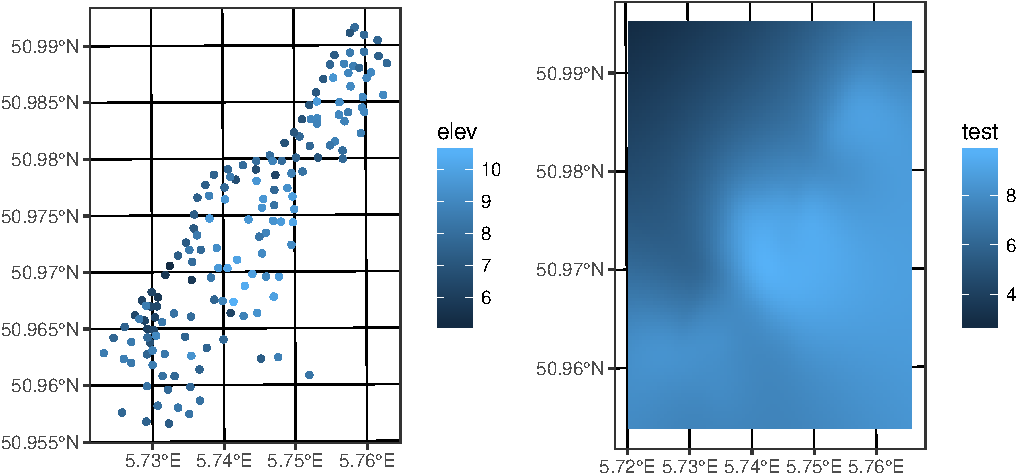
\includegraphics[width=\textwidth]{Lec16_files/figure-beamer/unnamed-chunk-49-1} \end{center}

\end{frame}

\end{document}
